\chapter{测试自动生成}

    现在, 有了OpenAPI规约语言描述的API行为文档, 和场景模型, 接下来的任务就是生成并执行测试. 测试的生成有两个层次: 一个是为单次API请求生成请求数据(即输入数据), 一个是将单个请求串联起来生成API执行序列作为测试用例.
    
    \section{数据定义表达}
    
        在场景模型的定义中, 数据定义方面的扩展主要为合法请求数据定义(式\ref{eq:scenario_model_state}的$in_q$), 合法响应数据定义(式\ref{eq:scenario_model_state}的$out_q$), 请求数据依赖定义(式\ref{eq:scenario_model_state}的$d_q$)和响应数据断言定义(式\ref{eq:scenario_model_state}的$a_q$). 此外, 状态转移的条件(式\ref{eq:scenario_model}的$\sigma_{\mathcal{A}}$)基于响应数据, 也可被视为数据定义的一部分. 其中, 除了状态转移的条件外, 其余数据定义均以集合的形式给出, 即定义了满足要求的合法数据的集合. 合法请求/响应数据的定义是直接给出集合, 请求数据依赖和响应数据断言的定义为一个返回这种集合的函数. 而状态转移的条件定义为单个数据实例, 但进行简并, 亦可视为直接给出集合, 即当响应数据属于定义的集合时可使用某项转移.
        
        测试自动生成以本文的场景模型作为基础, 场景模型抽象了API的使用模式, 并为生成高效的测试用例提供了必需知识. 其中, 数据定义与测试自动生成息息相关. 在生成请求数据时, 需要合法请求数据的定义与请求数据依赖的定义. 而在执行序列生成时, 需要合法响应数据与响应数据断言定义用于验证, 需要转移条件定义用于选择状态转移. 因此, 这些数据定义围绕着测试自动生成的需求进行表达.
        
        生成请求数据与合法请求数据定义, 请求数据依赖定义相关. 需求则是从满足这些定义的集合中随机选出一个合法元素作为生成的请求数据. 因此, 合法请求数据定义使用\textbf{JSON模式}(JSON Schema)或\textbf{自定义生成函数}表达, 请求数据依赖定义则使用\textbf{自定义生成函数}或\textbf{运行时表达式}(Runtime Expression)表达.
        
        响应数据验证与合法响应数据定义, 响应数据断言定义相关. 需求则是验证响应数据是否属于定义的集合. 因此, 合法响应数据定义使用\textbf{JSON模式}或\textbf{自定义校验函数}表达, 响应断言定义使用\textbf{运行时表达式}或\textbf{自定义校验函数}表达.
        
        选择状态转移时, 需要用到状态转移的定义, 需求也是验证响应数据是否属于定义的集合. 按照场景模型的定义, 定义的集合为一个固定的响应数据集合, 但为了增强场景模型的表达能力, 对定义进行了扩展, 允许集合与运行时状态序列相关, 即类似于响应数据断言定义. 因此, 它也可以使用\textbf{运行时表达式}和\textbf{自定义校验函数}表达.
        
        各个数据定义的可用表达方式总结于表\ref{tab:data_def_format}.
        
        \begin{table}[!htb]
            \centering
            \begin{tabular}{c||c|c|c|c}
                \toprule
                 & JSON模式 & 自定义生成函数 & 运行时表达式 & 自定义校验函数 \\
                \hline
                合法请求数据 & 可用 & 可用 & & \\
                \hline
                请求数据依赖 & & 可用 & 可用 & \\ 
                \hline
                合法响应数据 & 可用 & & & 可用 \\
                \hline
                响应数据断言 & & & 可用 & 可用 \\
                \hline
                状态转移条件 & & & 可用 & 可用 \\
                \bottomrule
            \end{tabular}
            \caption[各数据定义的可用表达方式表]{各数据定义的可用表达方式列表.}
            \label{tab:data_def_format}
        \end{table}
        
        \label{sec:set_define}
        
        \textbf{JSON模式}(JSON Schema)\footnote{https://tools.ietf.org/html/draft-wright-json-schema-validation-00}是一种定义严谨的结构化JSON数据描述格式. JSON模式本身是一段JSON数据体, 它详细定义了数据的类型, 取值范围, 包含的各个成员域, 各个子元素格式等等. 图\ref{fig:json_schema_example}展示了JSON模式的示例, 它定义了一个名为\texttt{Person}的组合数据类型, 该类型包括三个域, 分别为字符串类型的\texttt{firstName}, 字符串类型的\texttt{lastName}和非负整数类型的\texttt{age}, 其中\texttt{age}域为可选. 满足此格式定义的数据构成了一个集合. 当JSON模式用于定义合法请求数据时, 使用数据生成策略随机生成符合定义的请求数据, 详细讨论见\ref{sec:req_data_gen}小节. 当JSON模式用于定义合法响应数据时, 直接对响应数据使用定义的模式进行验证.
        \begin{figure}[!htb]
            \centering
            \scriptsize
            \tt
            
            \begin{lstlisting}[language=YAML]
{
    "title": "Person",
    "type": "object",
    "properties": {
        "firstName": {
            "type": "string"
        },
        "lastName": {
            "type": "string"
        },
        "age": {
            "description": "Age in years",
            "type": "integer",
            "minimum": 0
        }
    },
    "required": ["firstName", "lastName"]
}
            \end{lstlisting}
            
            \caption[JSON模式示例]{JSON模式示例.}
            \label{fig:json_schema_example}
        \end{figure}
        
        \textbf{自定义生成函数}是留给用户自定义的生成函数. 在生成测试数据时, 将当前序列所有之前的请求数据与响应数据传入函数, 该函数返回一个数据, 即为生成的测试数据. 定义良好的自定义生成函数应引入随机性, 并使用采样策略, 从满足合法性和依赖要求的数据集合中抽样出数据返回. 用户使用Python语言编写此函数, 并在场景脚本中指定模块名与函数名.
        
        \textbf{运行时表达式}(Runtime Expression)是表达部分简单的依赖关系的一种简便快捷的方法. 该方法由OpenAPI规约语言引入\footnote{https://swagger.io/specification/\#runtimeExpression}, 在本文场景模型的数据定义表达中则被广泛借鉴与采用. 运行时表达式用于明确指定一次API请求过程中的某一数据元素, 如:
        \begin{itemize}
            \item \texttt{\$request.body\#/user/identity}: 请求数据体的\texttt{user}域的\texttt{identity}域;
            
            \item \texttt{\$statusCode}: 响应状态码;
            
            \item \texttt{\$response.header.x-oss-acl}: 响应头的\texttt{x-oss-acl}域.
        \end{itemize}
        在本文中使用时, 使用状态名称列表(对应式\ref{eq:scenario_request_depen}的$q_d$)和列表中下标(对应式\ref{eq:scenario_request_depen}的$index_d$))确定是哪一个API请求, 再使用该表达式确定具体数据元素. 当其不满足OpenAPI定义的格式时, 则视为普通数据对象使用. 因此, 它可以十分方便地表达请求数据依赖, 响应数据断言和状态转移条件中与其他状态的数据的关联关系. 但是, 由于表达式仅指向一个确定的值, 故表达的也仅仅是单元素集合, 对于常使用的多元素集合则无能为力.
        
        \textbf{自定义校验函数}类似自定义生成函数, 是留给用户自定义的校验函数. 在验证是否满足条件时, 将当前序列所有之前与当前的请求数据与响应数据传入, 该函数返回一个布尔值, 表示是否满足函数定义的条件. 定义良好的自定义校验函数应是确定性的, 即对于传入的之前的请求数据和响应数据, 应存在一确定集合, 当前响应数据属于此集合时返回为真, 否则为假. 因此, 此函数定义了一确定集合, 故可用来表达合法响应数据定义, 响应数据断言定义和状态转移条件定义. 类似自定义生成函数, 用户使用Python语言编写此函数, 并在场景脚本中指定模块名与函数名.
        
    \section{请求数据生成}
        \label{sec:req_data_gen}
        
        请求数据的自动化生成, 在本文的场景模式中, 即为在对应数据定义集合中的采样. 上一小节总结了数据定义的表达方式, 与请求数据生成相关的数据定义有合法请求数据定义和请求数据依赖定义, 其中合法请求数据定义可用JSON模式和自定义生成函数表达, 请求数据依赖定义可用自定义生成函数和运行时表达式表达. 请求数据生成根据表达方式的不同采取不同方法.
        
        \begin{table}[!htb]
            \centering
            \begin{tabular}{rll}
                \toprule
                类型 & 条件 & 策略 \\
                \midrule
                null & / & 返回元素\texttt{Null} \\
                \hline
                integer \& & 存在\texttt{multipleOf}域 & 从满足倍数关系的值空间中采样 \\
                \cline{2-3}
                float & 存在\texttt{enum}域 & 从定义的有限集合中采样 \\
                \cline{2-3}
                & 存在\texttt{MIN}或\texttt{MAX}域 & 从定义的区间中采样 \\
                \cline{2-3}
                & / & 在对应类型的整个区间中采样 \\
                \hline
                boolean & 存在\texttt{enum}域 & 从定义的有限集合中采样 \\
                \cline{2-3}
                & / & 使用伯努利分布($p=0.5$) \\
                \hline
                string & 存在\texttt{regex}域 & 从正则表达式定义的模式中生成 \\
                \cline{2-3} 
                & 存在\texttt{enum}域 & 从定义的有限集合中采样 \\
                \cline{2-3}
                & \texttt{format}域存在 & 先随机日期, \\
                & 且为\texttt{'date'} & 再以RFC3339的full-date格式表示 \\
                \cline{2-3}
                & \texttt{format}域存在 & 先随机日期时间, \\
                & 且为\texttt{'datetime'} & 再以RFC3339的date-time格式表示 \\
                \cline{2-3}
                & \texttt{format}域存在 & \multirow{2}{*}{随机二进制串, 以\texttt{bytes}格式返回} \\
                & 且为\texttt{'binary'} &  \\
                \cline{2-3}
                & 存在\texttt{minLength} & 先从指定长度区间随机长度值, \\
                & 或\texttt{maxLength}域 & 再随机生成字符串 \\
                \cline{2-3}
                & \multirow{2}{*}{/} & 先随机确定长度值(默认不超过255),\\
                & & 再随机生成字符串 \\
                \hline
                array & 存在\texttt{maxItems} & 先从指定区间随机列表长度,\\
                & 或\texttt{minItems}域 & 再随机递归生成各元素 \\
                \cline{2-3}
                & \multirow{2}{*}{/} & 先随机确定列表长度,\\
                & & 再随机递归生成各元素 \\
                \hline
                object & / & 递归生成各成员 \\
                \bottomrule
            \end{tabular}
            \caption[JSON模式数据定义的生成策略表.]{JSON模式数据定义的生成策略表. 从JSON模式生成请求数据时, 依据基本类型和条件分类讨论, 采取不同策略.}
            \label{tab:schemagen}
        \end{table}
    
        当使用JSON模式表达时, 由于每个数据对象都属于JSON模式定义的基本类型之一, 因此, 进行分类讨论, 为每个基本类型设计并实现了采样策略. 对于一些常见的子类型如日期、时间、二进制串等, 以条件的形式定义了特殊采样策略. 具体策略见表\ref{tab:schemagen}. 特别地, 当多个条件均满足时, 则合理结合多个策略生成. 策略的设计以满足随机性且保证生成的数据合法为目标. 此外, 实际实现中, 允许用户以基本类型和\texttt{format}域分类, 使用扩展函数自定义策略.
        
        当使用自定义生成函数表达时, 将当前上下文, 即包括请求数据与响应数据的执行序列, 传入自定义函数, 由于函数期望的返回值就是其隐式定义的集合的采样, 故直接将返回值作为请求数据即可.
        
        当使用运行时表达式表达时, 首先对表达式进行解析, 如果确定其为合法的运行时表达式, 则根据其含义从执行序列中提取出指定的数据对象作为请求数据, 否则直接将其本身视为数据对象作为请求数据. 由于指定的元素是确定的, 而不是多元素集合, 故无需定义采样或生成策略.
        
        对某个请求数据的定义, 合法请求数据定义与请求数据依赖定义常常有所重叠, 即可能同时具有这两个定义, 甚至请求数据依赖的定义有多个. 这时, 生成的请求数据应要同时满足这多个定义的限制. 因此, 本文会优先根据请求数据依赖定义生成数据, 再检查其是否满足其余定义的要求, 如果不满足则多次随机尝试, 若尝试次数超过一定阈值(实现中为方便起见设定为100)则判定为定义间存在冲突, 报错并中断请求数据生成过程.
        
    \section{执行序列生成}
        如果以自动机的视角看待场景模型, 那么它所定义的也是合法串的集合以及它们的概率分布. 由于每个自动机的状态可以与一个API服务端点关联, 所以字符串也可以对应于API的响应序列. 在进行web API测试时, 一个这样的包含具体请求数据与响应数据的执行序列, 即是一个测试用例和它的一次执行结果.
        
        因此, 执行序列生成算法基本上就是场景模型的一次工作过程. 与自动机不同的是, 自动机在工作之前, 输入串是给定的, 而场景模型的串则由工作时每个状态上API调用的响应数据组成, 是一边工作一边动态生成的. 这也对应了测试用例的生成与执行在本文的方法中是一个整体, 同时进行的.
        
        执行序列生成算法大体流程的伪代码如算法\ref{algo:seqgen}所示.
        
        \begin{algorithm}
          	\scriptsize
          	
            \caption{API执行序列生成算法}
          	
            \KwIn{$Spec$, $\mathcal{A}$} 
            \tcp{输入: API定义脚本和场景模型脚本}
            \tcp{场景模型$\mathcal{A} := \langle Q_{\mathcal{A}}, \Sigma, \sigma_{\mathcal{A}}, I_{\mathcal{A}}, F_{\mathcal{A}}, P_{\mathcal{A}}\rangle$}
            \KwOut{$r$, $T$}
            \tcp{输出: 执行序列和终止原因}
            $q$ $\gets$ RandomChoice($Q_{\mathcal{A}}$, $I_{\mathcal{A}}$)\;
            \tcp{根据初始状态概率分布函数随机初始状态$q := \langle t_q, in_q, out_q, d_q, a_q\rangle$}
            $current$ $\gets$ $EmptyMap$\;
            $current.state$ $\gets$ $q$\;
            $r$ $\gets$ $EmptyList$\;
            $stop$ $\gets$ $false$\;
            \While {$\neg stop$} {
            	$i$ $\gets$ $EmptyMap$\;
                $o$ $\gets$ $EmptyMap$\;
            	\If(\tcp*[h]{$q$有关联的API服务端点}) {$t_q \neq empty$}{
                	\ForEach(\tcp*[h]{遍历处理所有请求参数}) {$param$ in $t_q.params$} {
                    	\If(\tcp*[h]{当前参数$param$有数据依赖, 则从依赖生成请求数据}) {$d_q.param \neq Null$} {
                        	$d$ $\gets$ $d_q.param$\;
                            \tcp{数据依赖$d := \langle q_d, index_d, f_d\rangle$}
                            $q'$ $\gets$ PickDependee($r$, $q_d$, $index_d$)\;
                            $i.param$ $\gets$ RandomFromSet($f_d(i_{q'}, o_{q'})$)\;
                        } \Else(\tcp*[h]{当前参数$param$无数据依赖, 则默认从合法请求集合中生成请求数据}) {
                        	$i.param$ $\gets$ RandomFromSet($in_q.param$)\;
                        }
                    }
                    $o$ $\gets$ Request($Spec.t_q$, $i$)\;
                    \tcp{发送请求, 并解析返回的响应}
                    $current.i$ $\gets$ $i$\;
                    $current.o$ $\gets$ $o$\;
                    \If(\tcp*[h]{请求失败}) {RequestFail($o$)} {
                    	$T$ $\gets$ ``Request Fail''\;
                        $stop$ $\gets$ $true$\;
                    } \Else(\tcp*[h]{请求成功}) {
                    	\ForEach(\tcp*[h]{遍历返回的响应的各个域}) {$field$ in $t_q.fields$} {
                        	\If(\tcp*[h]{响应的$field$域有断言定义, 则验证是否满足断言}) {$a_q.field \neq Null$} {
                            	$a$ $\gets$ $a_q.field$\;
                                \tcp{响应断言$a := \langle q_a, index_a, f_a\rangle$}
                                $q'$ $\gets$ PickDependee($r$, $q_a$, $index_a$)\;
                                \If {$o.field \notin f_a(i_{q'}, o_{q'})$} {
                                	$T$ $\gets$ ``Response Assert Fail''\;
                                    $stop$ $\gets$ $true$\;
                                }
                            }
                            \If(\tcp*[h]{响应的$field$域有合法响应定义, 则验证是否满足之}) {$out_q.field \neq Null$} {
                            	\If {$o.field \notin out_q.field$} {
                                	$T$ $\gets$ ``Response Illegal Fail''\;
                                    $stop$ $\gets$ $true$\;
                                }
                            }
                        }
                    }
                }
                $r$.append($current$)\;
                \If {$\neg stop$} {
                	$\chi$ $\gets$ RandomNumber($U(0,1)$)\;
                    \If(\tcp*[h]{依照终止概率分布函数决定是否终止执行}) {$\chi \le F_{\mathcal{A}}(q)$} {
                    	$T$ $\gets$ ``Final State''\;
                        $stop$ $\gets$ $true$\;
                    }
                }
            	\If(\tcp*[h]{继续执行, 依照转移概率分布函数选择转移边}) {$\neg stop$} {
                	$q$ $\gets$ RandomChoice($\sigma_{\mathcal{A}}(q,o)$, $P_{\mathcal{A}}(q,o) / \left(1 - F_{\mathcal{A}}(q)\right)$)\;
                    $current$ $\gets$ $EmptyMap$\;
                    $current.state$ $\gets$ $q$\;
                }
            }
            \Return {$r$, $T$}

            \label{algo:seqgen}
        \end{algorithm}
        
        在此算法中, 首先, 根据初始状态概率分布函数$I_{\mathcal{A}}$随机选择初始状态. \texttt{RandomChoice()}函数接受两个列表作为参数, 分别表示候选元素和每个元素的概率权重, 它按照权重随机抽取一个元素作为返回值, 故\texttt{RandomChoice(}$Q_{\mathcal{A}}$\texttt{,}$I_{\mathcal{A}}$\texttt{)}返回随机选择的初始状态. 这个初始状态记录在变量$q$中. 然后, 算法在场景模型上正式开始工作, 对应于代码中的大循环"\textbf{while} $\neg stop$ \textbf{do}", 其中$stop$记录了在某一步结束后是否终止执行, 初始化为$false$. 
        
        每一步中, 使用$current$记录当前所处状态, 请求数据和响应数据等上下文信息. $r$是存储整个序列的上下文信息的总列表. 如果当前状态与一个API服务端点相关联($t_q \neq empty$), 算法将遍历请求数据的各个参数定义, 分别对各个参数运行\ref{sec:req_data_gen}小节描述的请求数据生成算法, 生成的请求数据记录在变量$i$中. 之后, 算法发送请求并解析响应数据, 发送请求时除了需要给出API的名称$t_q$和请求数据$i$外, 还需要结合OpenAPI语言编写的API描述脚本获取必需的要素, 此处用$Spec.t_q$代指这些要素. 解析出的响应数据记录在变量$o$中. 若请求发送失败或响应数据解析失败, 执行终止. 否则, 解析完成后, 算法扫描响应数据的各个域. 对每个域, 首先检测其是否定义对应的响应断言, 如果有, 则对断言函数求值, 求得断言定义的集合, 并验证当前域的数据是否在此集合内, 若不在则执行终止. 然后, 再检测其是否定义对应的合法响应集合, 如果有, 则直接获取这个合法响应集合, 并验证当前域的数据是否在此集合内, 若不在亦执行终止.
        
        如果此时执行尚未终止, 则进行转移决策. 转移决策部分决定是否在当前状态处正常终止或是选择某条转移边转移到另一状态. 首先, 从$[0,1]$的均匀分布中抽取一随机数$\chi$, 若$\chi \le F_{\mathcal{A}}(q)$($q$为当前状态), 则表明随机的结果是在当前状态处正常终止, 那么终止即可. 否则, 需要进行状态转移, 将当前状态$q$与响应数据$o$部分应用到转移概率分布函数$P_{\mathcal{A}}$, 得到的$P_{\mathcal{A}}(q,o)$建立了从合法转移的目标状态到其概率分布的映射. 由于之前已经以$1 - F_{\mathcal{A}}(q)$的概率选择不终止, 此处选择某条转移的概率应为条件概率
        \begin{equation}
            P(\text{转移到}q' | \text{不终止}) = \dfrac{P(\text{转移到}q')} {P(\text{不终止})} = \dfrac{P_{\mathcal{A}}(q,o,q')} {1 - F_{\mathcal{A}}(q)}.
        \end{equation}
        故调用函数\texttt{RandomChoice(}$\sigma_{\mathcal{A}}(q,o)$\texttt{,}$P_{\mathcal{A}}(q,o)/\left(1-F_{\mathcal{A}}(q)\right)$随机选择下一步状态. 开始下一步的执行.
        
        当算法结束时, 返回的值包括执行序列$r$和终止原因$T$, 其中执行序列$r$详细记录了每一步的状态名称, 请求数据和响应数据, 终止原因$T$详细记录了执行终止的位置和具体信息, 便于确定测试用例的执行是否成功, 以及不成功的具体原因.
        
        算法结合了执行序列的生成和执行过程, 并且生成过程实时受执行结果(即API响应数据)的反馈影响. 序列生成是动态的, 这使预处理相关的加速和优化变得困难, 但也使生成的序列更为灵活, 更为贴近实际使用场景.
        
    \section{启发式执行序列生成}
        除了以上提出的算法, 本文亦探索了启发式的执行序列生成. 启发式的改进主要在转移边的选择方面. 在以上算法中, 转移边的选择直接继承了概率有限状态自动机的方式, 严格按照定义的概率权值, 然而, 在运行此算法多次生成多个测试用例时, 为了提高测试覆盖率, 可以不必拘泥于定义的权值, 而进行一定的调整.
        
        在此场景模型中, 测试覆盖率常常与场景的状态覆盖率, 转移覆盖率, 以及综合路径覆盖率正相关. 一个基本的思想便是将这些覆盖率的提升期望加入考虑, 对提升这些覆盖率幅度较大的转移边增大选择概率.
        
        一种贪心策略是优先选择连接到未访问状态的转移边, 或直接选择未访问的转移边. 但是, 本文的实验发现, 由于场景模型目前采用人工设计, 包含的状态数和转移边数较少, 因此少量测试用例即可完全遍历, 故价值不大. 其他更复杂的启发式策略很可能会有效, 如考虑连续状态序列或整体路径的覆盖率等, 这有待进一步实验证实.
        
        另一方面, 启发式改进的直接作用亦可能并不显著. 虽然不使用启发式算法时, 测试用例冗余度较高, 即单位用例覆盖率不够高. 但受益于全自动生成的过程, 同等时间下, 生成测试用例的数目很大, 这可在一定程度上弥补甚至逆转总覆盖率的劣势. 具体结论需要依据具体场景模型进行评估, 是值得进一步探讨的问题.
    
    % extended version
    % \section{*启发式优化}
    %     \subsection{启发式执行序列生成}
    %     将上个小节移到本章来
    %     \subsection{启发式场景优化}
    %     不知道有冇时间做了

    \section{实验与评估}

        \label{sec:experiment}

        依靠实现的工具, 本文在三个实际的web API服务上进行了实验, 从四个方面评估了测试自动生成方法: 测试用例多样性, 测试覆盖率, 故障检测能力, 以及测试效率.
    
        \subsection{实验配置}
            \subsubsection*{云对象存储服务(OSS)}
                实验选择的第一个被测系统为合作研究组正在开发的云对象存储服务(OSS)系统(版本1.0)(后文简称\textbf{OSS}). 此服务提供了33个web API接口, 并有较完整的使用文档. 测试时, 期望所有的API和功能点均业已实现完成.
                
                最近以来, 云对象存储服务(OSS)已经成为了流行的云存储服务形式. 许多大型云服务提供商均已提供云对象存储服务, 如亚马逊AWS\footnote{https://aws.amazon.com/s3}, IBM云\footnote{ https://console.bluemix.net/catalog/services/cloud-object-storage}和阿里云\footnote{ https://www.alibabacloud.com/product/oss}等. 在云对象存储服务中, 每个账号, 在每个服务器区域, 都可以有许多存储空间(bucket). 存储空间(bucket)与文件系统中的文件夹类似, 对象(object)与文件系统中的文件类似. 用户可以上传对象, 删除对象, 重命名对象, 创建符号链接等等. 每个对象都属于一个固定的存储空间.
                
                对于云对象存储服务, 本工作首先为这33个API编写了OpenAPI格式的API行为描述脚本. 然后, 设计了一些小型场景模型来检验每个API的基本功能. 在此之后, 设计了三个较大型的综合场景模型Scenario A、Scenario B、Scenario C以进行综合测试, 这三个场景均与实际使用场景较相似, 测试用例的生成与执行期望能够模拟实际部署后的高负载环境. 对于每个场景, 运行实现的工具随机生成并执行了1,000个测试用例. 所有3,000个测试用例的执行与生成共耗时约4h, 这些用例及其执行结果都被妥善保存. 后续分析时, 在所有测试用例上进行统计, 未进行任何遴选.

                三个综合场景模型的直观表示详见图\ref{fig:oss_scenario_A}, 图\ref{fig:oss_scenario_B}和图\ref{fig:oss_scenario_C}. 状态S为这些场景的确定性初始状态, 状态T为这些场景的确定性终止状态. 在这三幅图中, 绿色表达式表示状态关联的请求数据依赖; 蓝色表达式表示状态转移的条件; 红色文字表示响应数据断言; 紫色文字为其它控制流说明.

                \begin{figure}
                    \centering
                    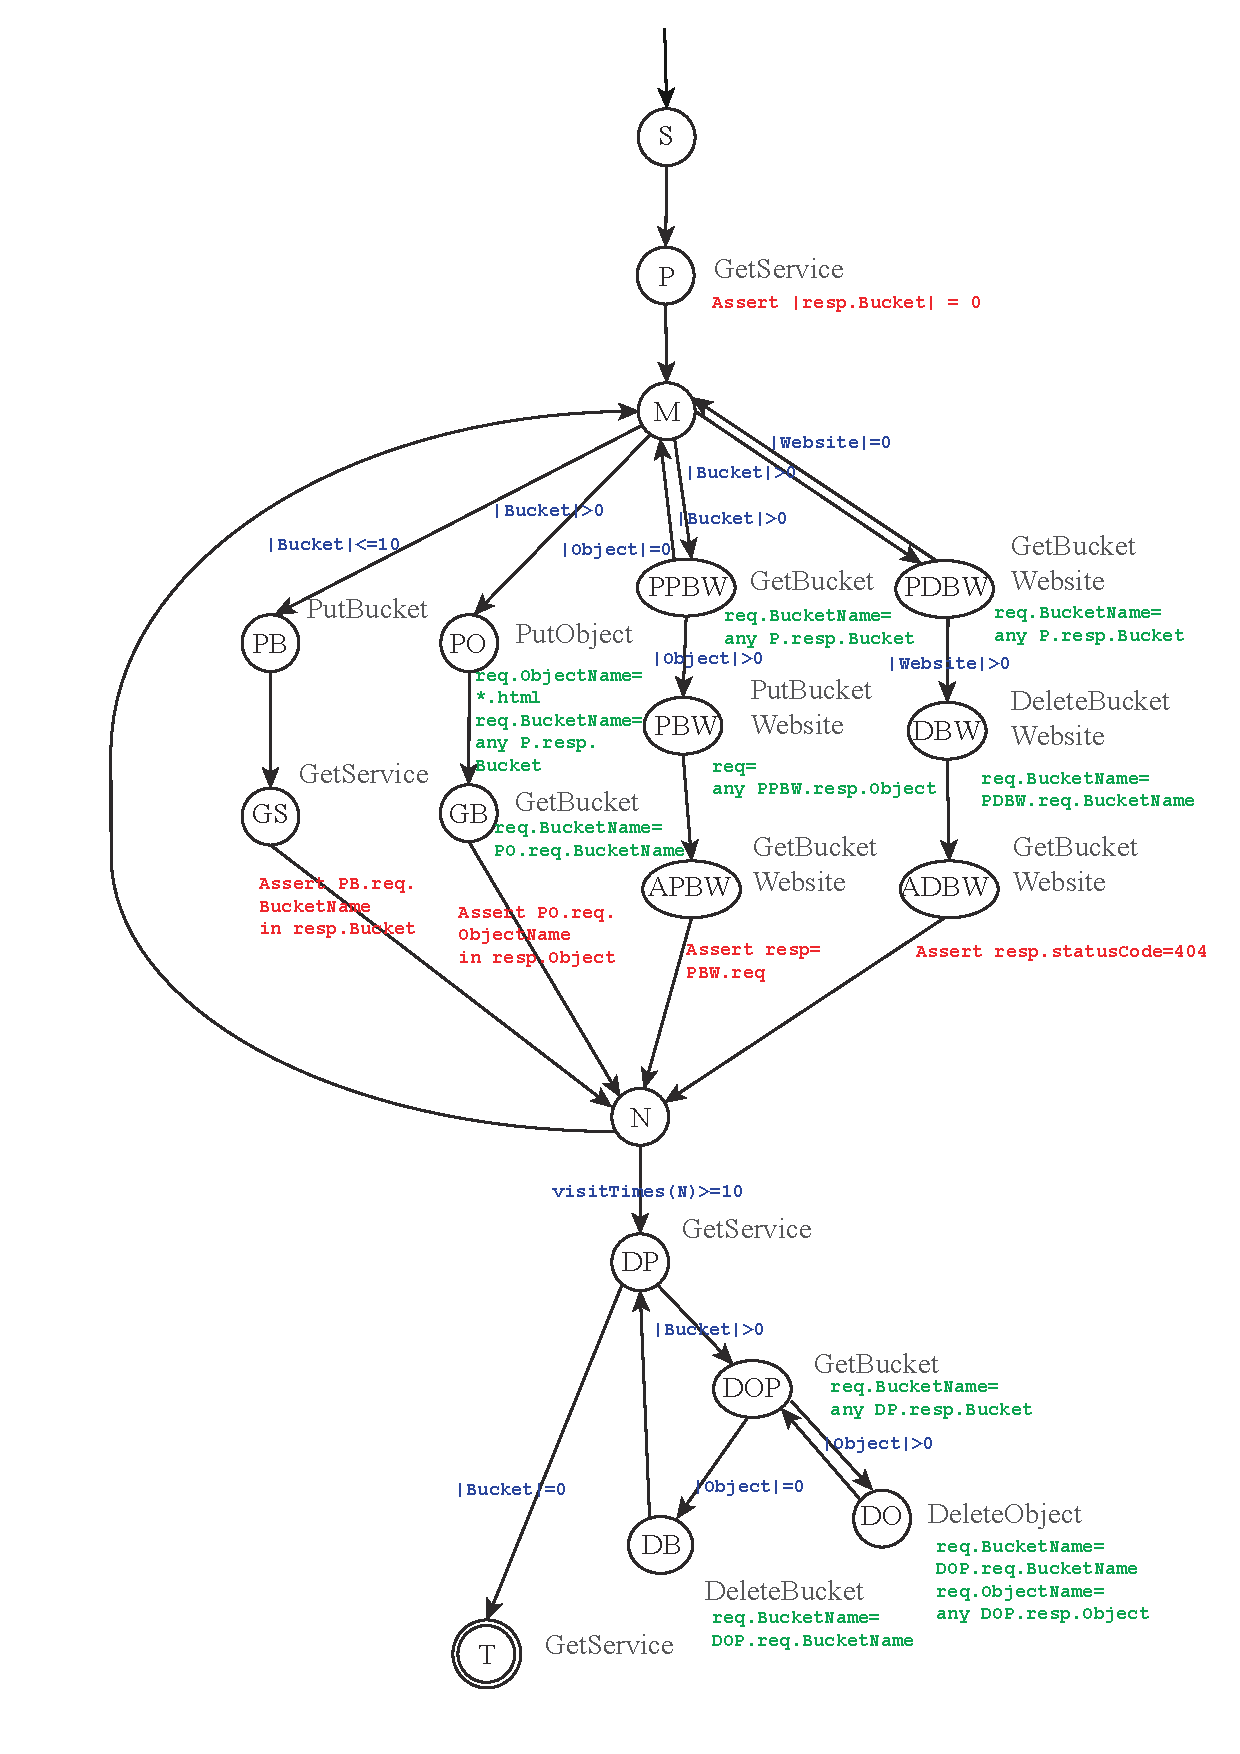
\includegraphics[width=400pt]{scenarioOSS_A_new.pdf}
                    \caption[云对象存储服务Scenario A]{OSS(云对象存储服务) Scenario A模型的直观表示.}
                    \label{fig:oss_scenario_A}
                \end{figure}
                
                 \begin{figure}
                    \centering
                    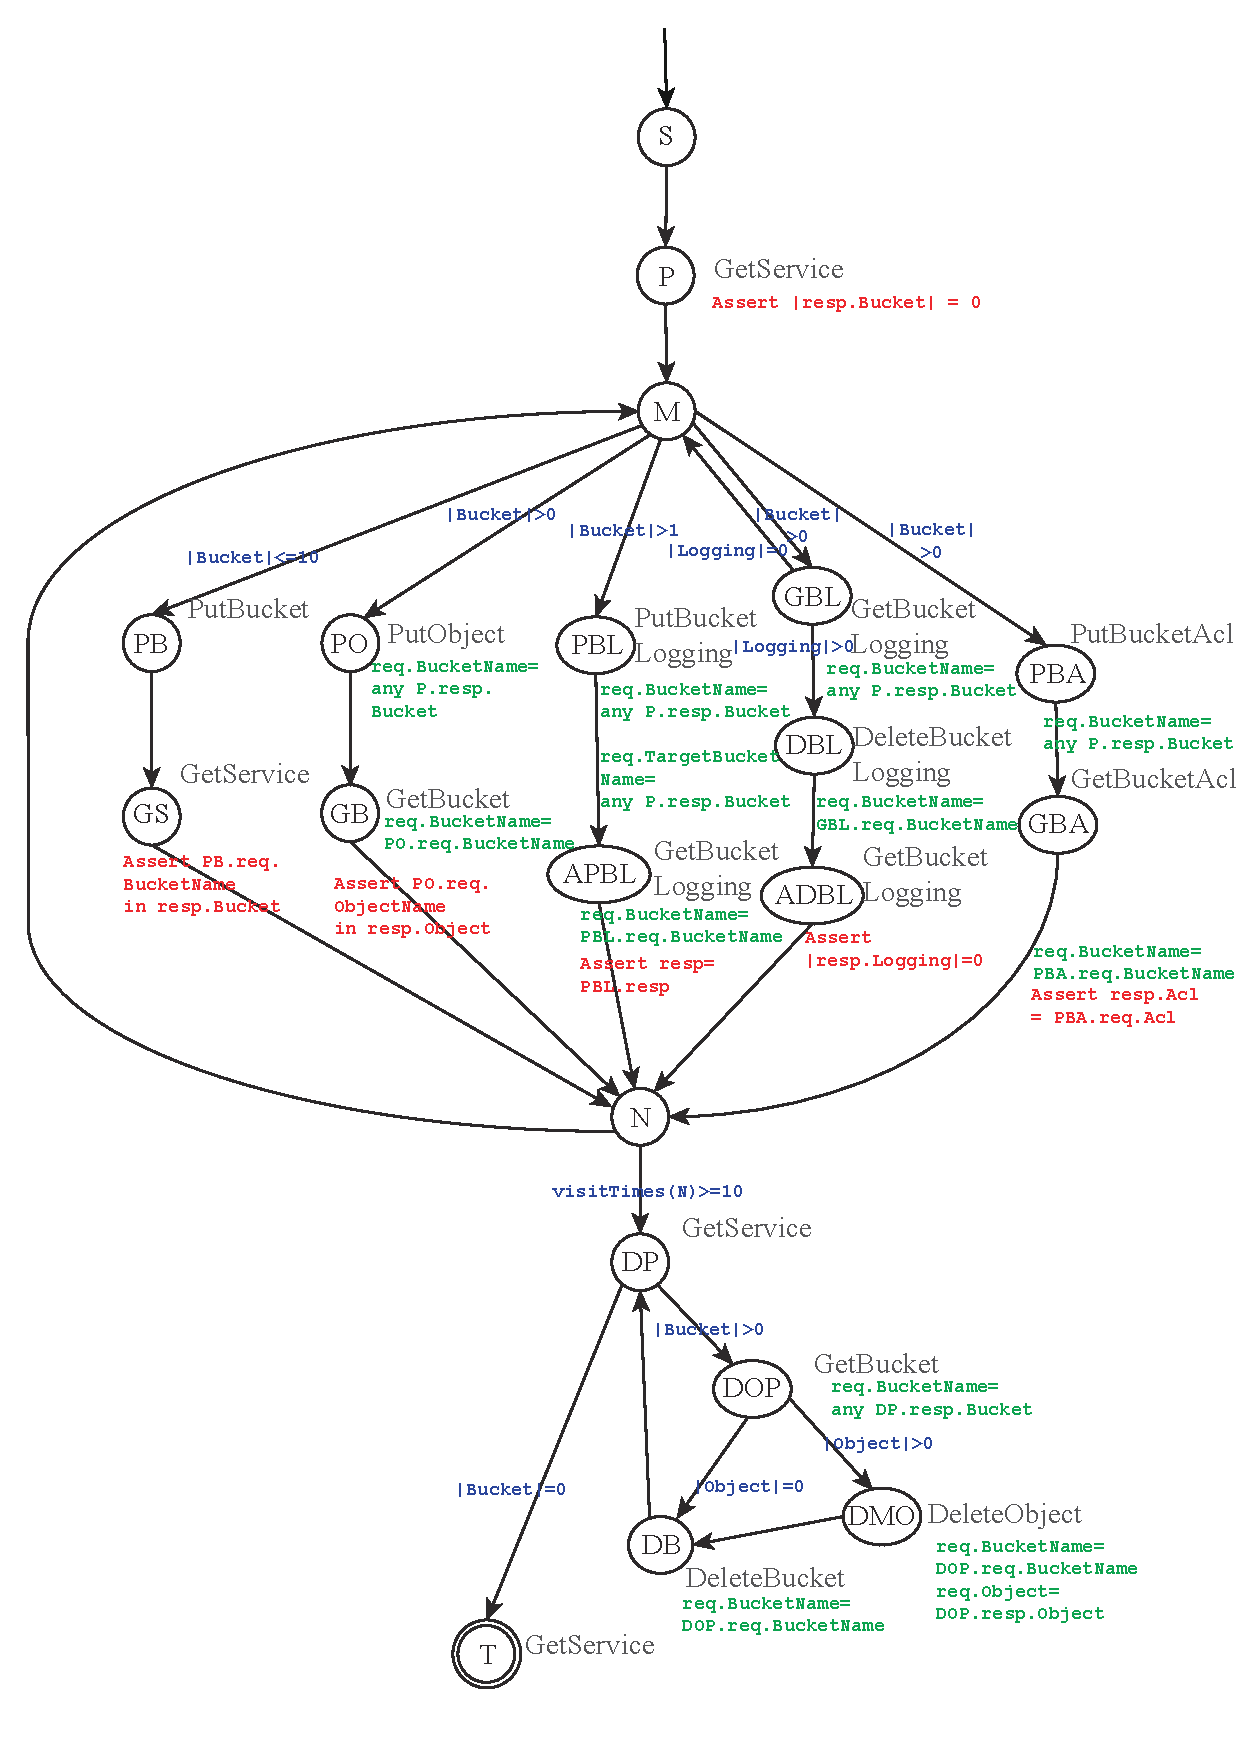
\includegraphics[width=400pt]{scenarioOSS_B_new.pdf}
                    \caption[云对象存储服务Scenario B]{OSS(云对象存储服务) Scenario B模型的直观表示.}
                    \label{fig:oss_scenario_B}
                \end{figure}
                
                 \begin{figure}
                    \centering
                    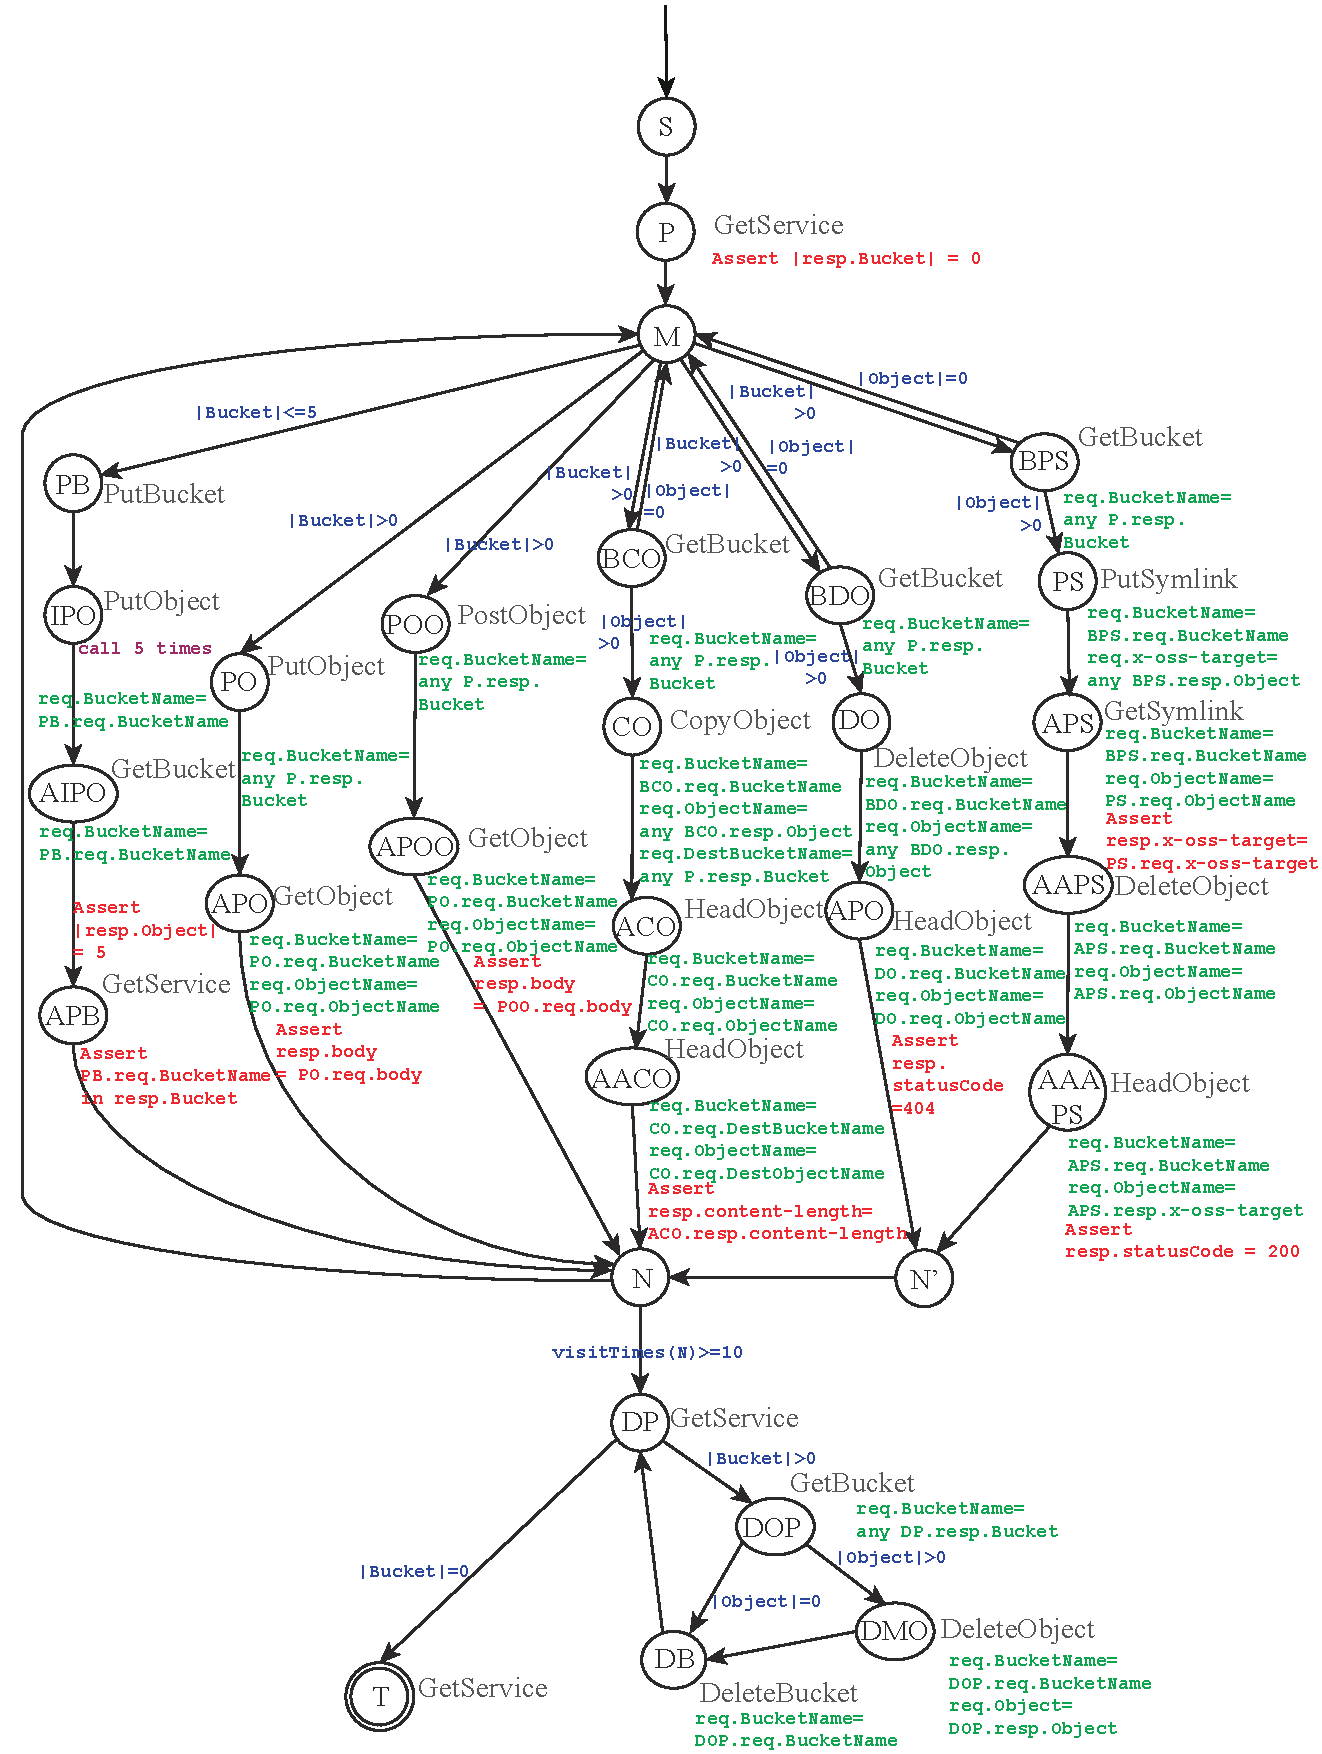
\includegraphics[width=450pt]{scenarioOSS_C_new.pdf}
                    \caption[云对象存储服务Scenario C]{OSS(云对象存储服务) Scenario C模型的直观表示.}
                    \label{fig:oss_scenario_C}
                \end{figure}
            
            \subsubsection*{云服务器服务(ECS)}
                第二个被测系统为某知名商业云计算提供商的云服务器(ECS)服务(后文简称\textbf{ECS}), 诸多大型应用均依托此提供商提供计算支持. 
                
                本实验测试它为普通用户提供的云计算实例租用服务, 相关接口共有26个, 均为web API, 并配有详细用户使用文档. 在此服务中, 用户可以租用实例, 退租实例, 获取实例运行状态, 启动实例, 关闭实例, 重启实例等等. 我们选择了其中8个web API, 编写了行为描述脚本, 然后设计了包含所有这8个web API的综合场景模型进行测试. 一共随机生成并执行了100个测试用例, 所有测试用例在进行统计与分析时均纳入考虑.

                综合场景模型的直观表示见图\ref{fig:ecs_scenario}. 在综合场景模型中, 状态Start为确定性初始状态, 状态T为确定性终止状态. 在图中, 请求数据依赖在状态关联的方框中写出; 状态转移的条件则标在转移边上, 其中方括号"$\left[\right]$"中的数字表示该转移的响应状态码条件; 该场景无响应数据断言.
        
                \begin{figure}[!htb]
                    \centering
                    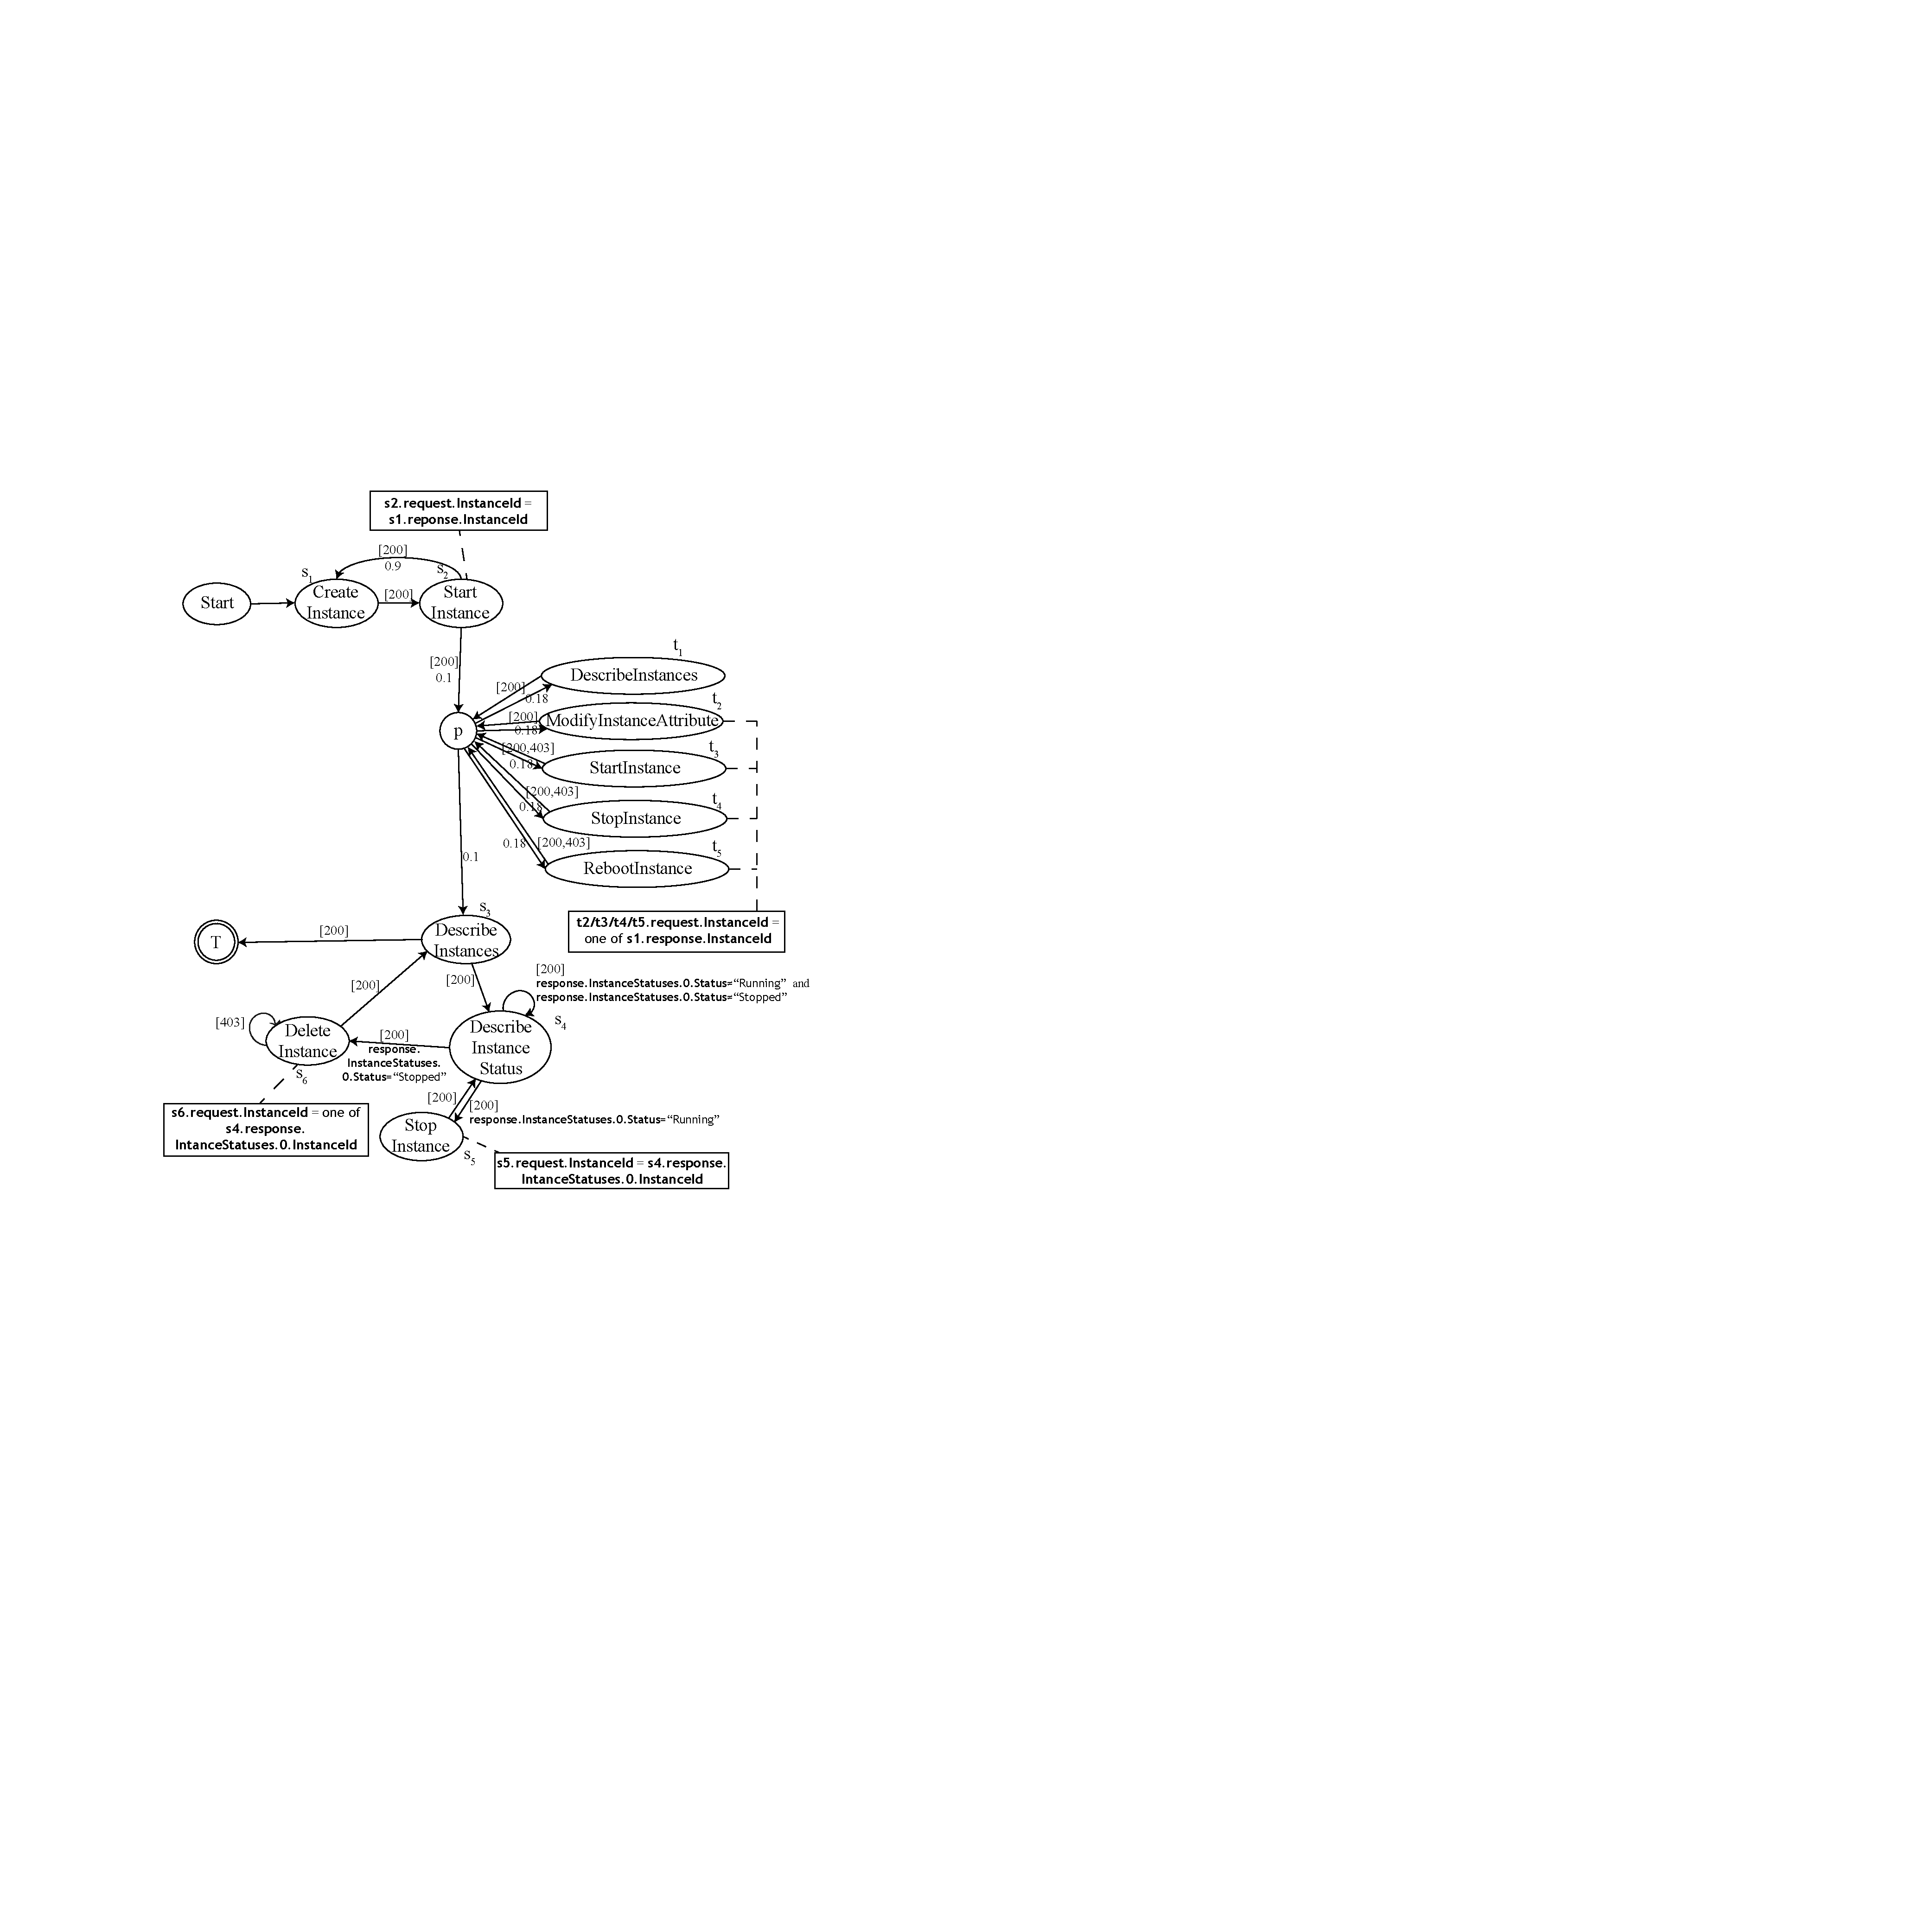
\includegraphics[width=400pt]{scenarioECS.pdf}
                    \caption[云服务器服务综合场景模型]{ECS(云服务器服务)的综合场景模型的直观表示.}
                    \label{fig:ecs_scenario}
                \end{figure}
            
            \subsubsection*{电子支付服务实时贷记API接口(E-payment)}
                \label{sec:epayment_setup}
                第三个被测系统是工业界合作团队提供的电子支付服务(后文简称\textbf{E-payment}). 本实验测试它的实时贷记API接口. 此API仅用于系统内部使用, 是微服务之间的通信接口, 因此使用LAN上的定制协议交互. 作为电子支付接口, 此服务拥有很高的可用率与很低的容错率要求. 同时, 它有多达20个参数. 由于模拟环境的缺失, 在本实验中, 暂未进行实际的调用与发送, 而是根据接口描述文档进行测试用例和请求数据的生成, 来验证生成的测试用例可以有效覆盖参数组合, 从而验证其在这类服务的测试上的可用性.
                
                E-payment服务(电子支付服务实时贷记API)的测试场景为链式, 该链式场景专用于分区测试数据的合成. 除了最后一个状态的其余状态均依次进行各个参数的生成, 为了引入数据分区, 各个参数的生成使用自定义生成函数, 自定义生成函数依照各个参数的数据分区随机生成参数. 最后一个状态对之前各个状态生成的参数进行合成, 即把各个参数合成为一个对象类型, 其各成员为之前生成的各参数, 此处引入数据依赖, 以从上下文中获取之前生成的参数. 最后一个状态与被测API关联, 发送合成对象作为请求数据. 示意图见\ref{fig:epayment_scenario}.
        
                \begin{figure}[!htb]
                    \centering
                    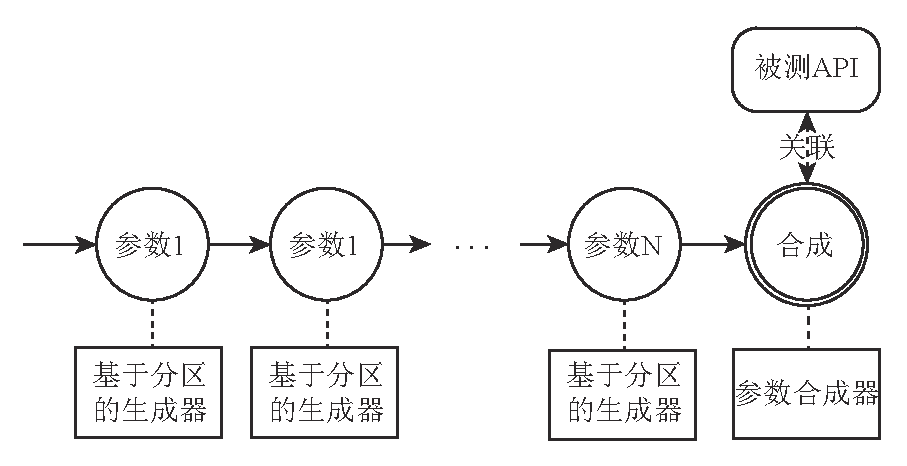
\includegraphics[width=400pt]{scenario_E-payment_pattern_new.pdf}
                    \caption[E-payment的场景模型示意图]{E-payment的场景模型示意图. 该场景被设计为链式, 专用于分区测试数据的合成.}
                    \label{fig:epayment_scenario}
                \end{figure}

                利用此场景模型, 花费数小时生成了巨量(超过两百万个)的测试用例, 并计算了这些测试用例对于参数分区的全组合的覆盖率. 这种方式不仅仅评估了测试用例的覆盖率, 也检验了工具原型的鲁棒性和性能.

            \subsubsection*{实验配置小结}
                三个被测系统分别独立设计场景模型并进行实验. 使用它们的出发点与实验的侧重点也各有不同. 在表\ref{tab:sut_summary}中, 对各被测系统进行了简单对比与小结.

                \begin{table}[!htb]
                    \centering
                    \begin{tabular}{ccccc}
                        \toprule
                            被测系统名称 & 简称 & 设计场景数 & 被测API数 & 使用目的 \\
                        \midrule
                            & \multirow{4}{*}{OSS} & \multirow{4}{*}{3} & \multirow{4}{*}{33} & 测试用例多样性分析 \\
                            云对象存储服务 & & & & 覆盖率分析\\
                            原型系统 & & & & 故障检测能力分析\\
                            & & & & 测试用例多样性分析\\
                            \hline
                            某商业云 & \multirow{2}{*}{ECS} & \multirow{2}{*}{1} & \multirow{2}{*}{8} & 测试用例多样性分析 \\
                            服务器服务 & & & & 故障检测能力分析 \\
                            \hline
                            电子支付服务 & \multirow{2}{*}{E-payment} & \multirow{2}{*}{1} & \multirow{2}{*}{1} & \multirow{2}{*}{覆盖率分析} \\
                            实时贷记接口 & & & & \\
                        \bottomrule
                    \end{tabular}
                    \caption[被测系统总结表]{实验使用的三个被测系统的简单对比与小结.}
                    \label{tab:sut_summary}
                \end{table}

            
        \subsection{测试用例多样性}
            富有多样性的测试用例是本文测试方法追求的目标之一. 多样性保证了测试用例集构成的测试套件具有较高的覆盖率和较低的冗余度. 另一方面, 使用被测系统的用户形形色色, 实际的系统负载也十分富有多样性, 因此, 富有多样性的测试用例, 除了在测试质量高外, 在某种程度上也能说明生成它们的测试场景模型可以很好地表达使用场景.
            
            在web API的测试中, 由于测试用例指包含数据的API调用序列, 一种典型的多样性衡量指标便是调用序列的多样性. 如果测试用例的调用序列富有多样性, 那么测试用例也就富有多样性. 调用序列的多样性可以通过一系列测试用例中总API调用次数以及某一主要被测API的调用次数的\textbf{分布}反映出来.

            形式化地, 对某个测试用例, 设其调用/请求序列为$seq$, 则API总调用次数即为序列的长度$|seq|$, 某主要被测API $a$的调用次数为
            \begin{equation}
                |\left\{i | i \in seq, i._{API} = x \right\}|.
            \end{equation}
            这里考察的, 也就是对于生成的一系列测试用例, 这两类值的分布.
            
            \begin{figure}[!htb]
                \begin{minipage}{0.5\textwidth}
                    \centering
                    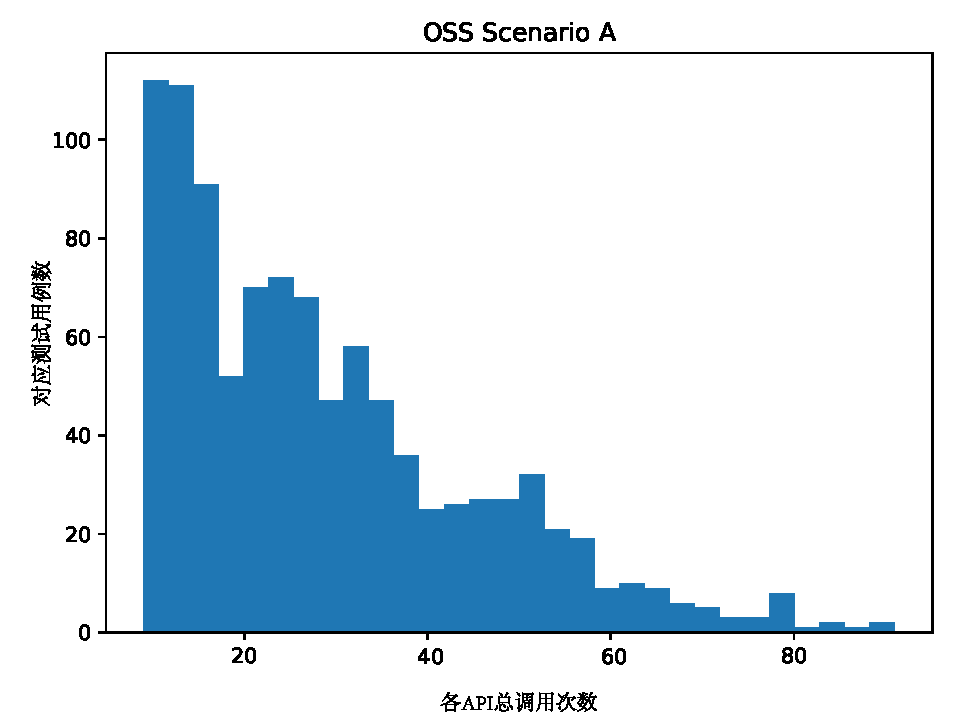
\includegraphics[width=200pt]{OSS_A_APICalls_cn.pdf}
                    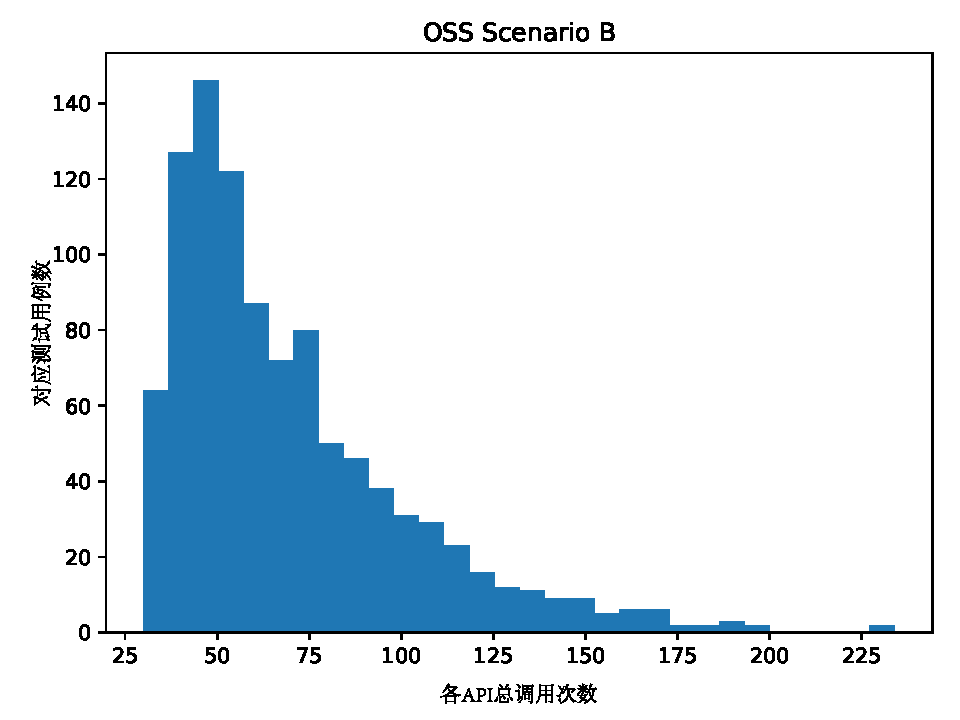
\includegraphics[width=200pt]{OSS_B_APICalls_cn.pdf}
                    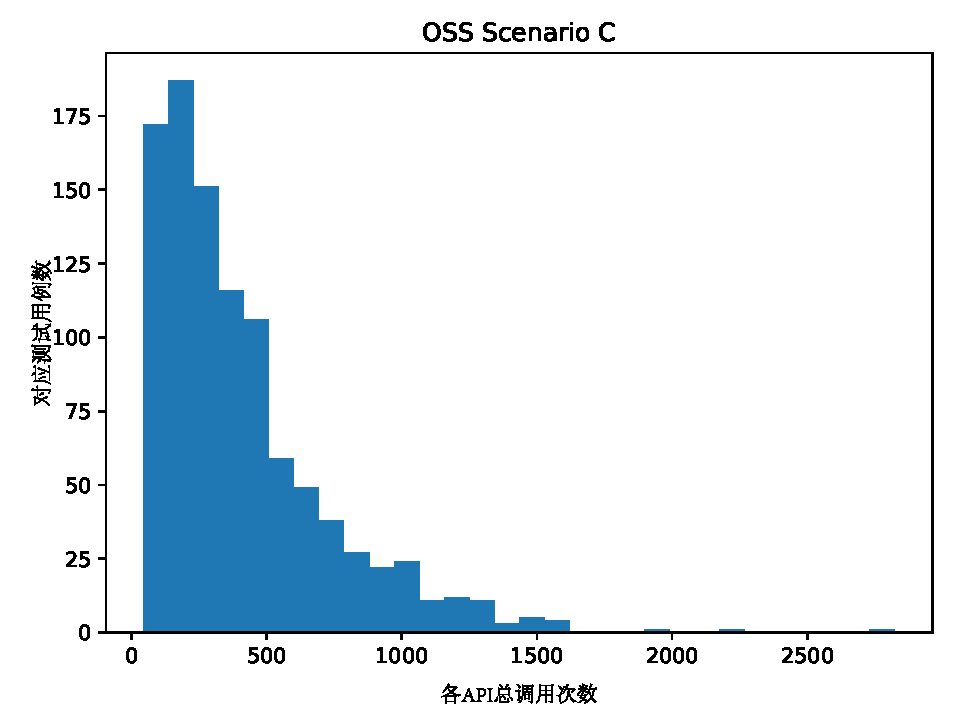
\includegraphics[width=200pt]{OSS_C_APICalls_cn.pdf}
                \end{minipage}
                \begin{minipage}{0.5\textwidth}
                    \centering
                    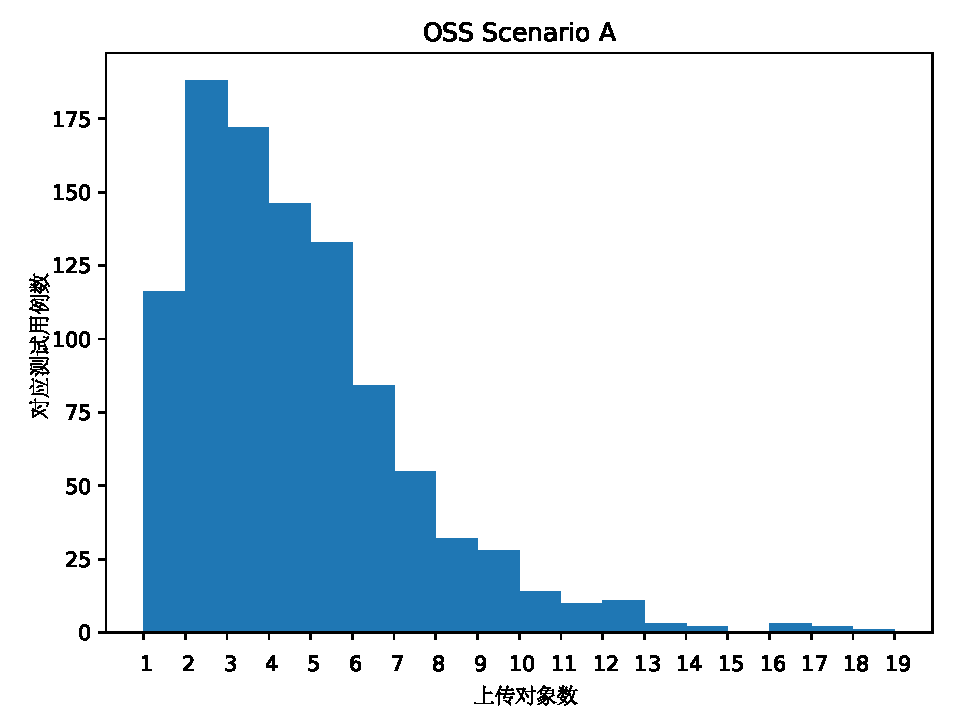
\includegraphics[width=200pt]{OSS_A_UploadedObj_cn.pdf}
                    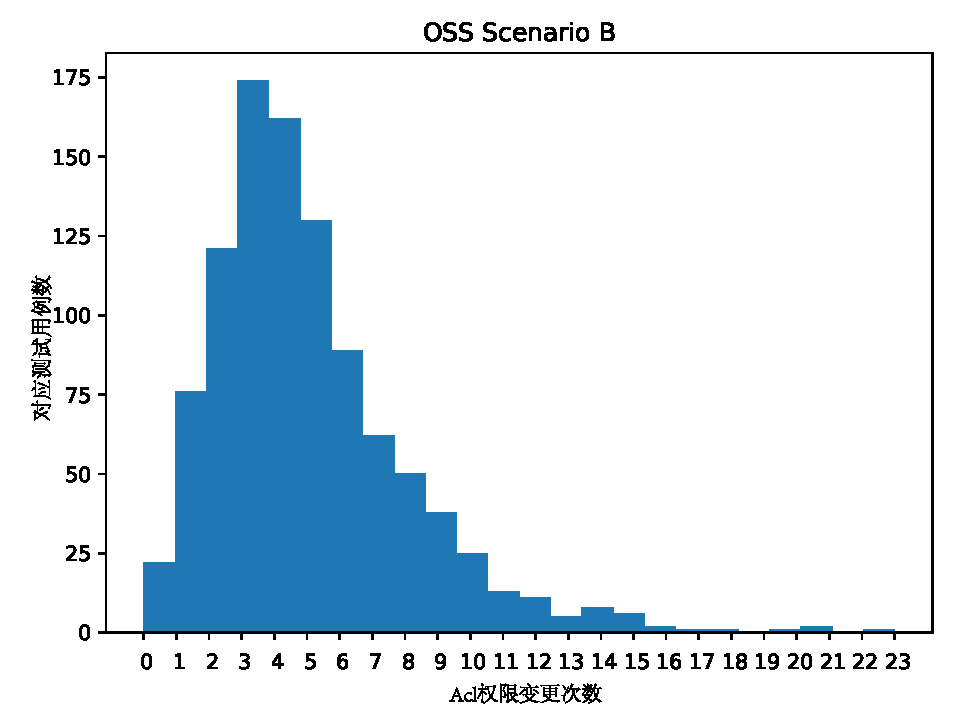
\includegraphics[width=200pt]{OSS_B_AclChange_cn.pdf}
                    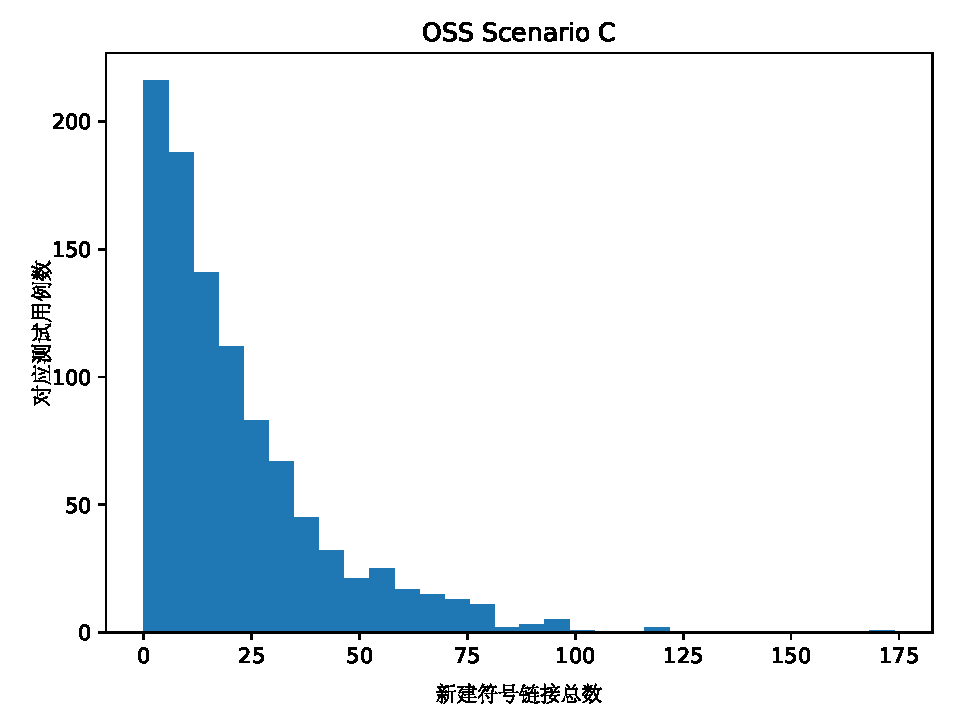
\includegraphics[width=200pt]{OSS_C_Putsymlink_cn.pdf}
                \end{minipage}
                \caption[OSS测试用例API调用次数分布直方图]{OSS测试用例操作次数分布直方图. 基于Scenario A, Scenario B, Scenario C三个场景生成的1,000个测试用例. 左侧为每个测试用例调用API总次数分布直方图, 右侧为对每个场景选取一种典型被测API, 其调用次数的分布直方图.}
                \label{fig:OSS_stat}
            \end{figure}
            
            \begin{figure}[!htb]
                \centering
                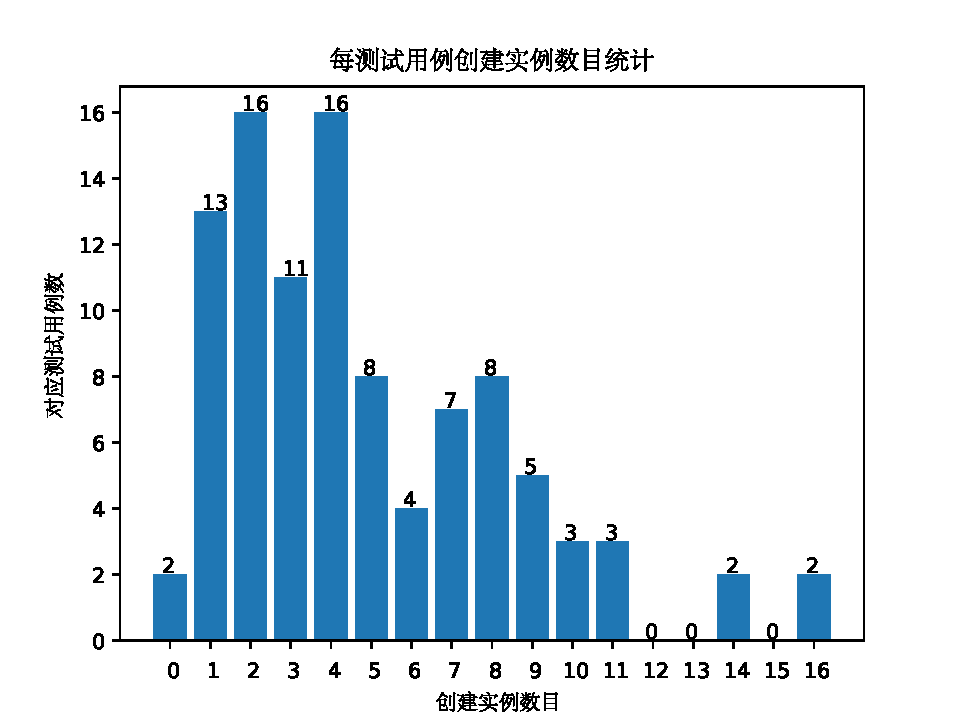
\includegraphics[width=400pt]{EC_instance_distribution_cn.pdf}
                \caption[ECS测试用例实例创建数分布直方图]{ECS测试用例实例创建数分布直方图, 也即创建实例API的调用次数分布图. 基于ECS测试场景生成的100个测试用例.}
                \label{fig:ECS_stat}
            \end{figure}
            
            图\ref{fig:OSS_stat}反映了对于OSS服务, 生成的测试用例的总API调用次数和主要被测API调用次数的统计分布直方图. 图\ref{fig:ECS_stat}反映了对于ECS服务, 生成的测试用例的创建实例数(即创建实例API调用次数)的统计分布直方图. 在这些直方图中, 横坐标为总API或某单个API的调用次数, 纵坐标为对应这个调用次数的测试用例数目. 虽然由于不同API在场景中所处位置不同的原因, 每幅直方图中的分布区间差异较大, 但是整体分布模式是类似的, 即无论是API总调用数目, 单API调用数目, 还是实例创建数目, 分布均较发散. 这反映了生成的测试用例的多样性.
            
            使用变异系数(CV, Coefficient of Variation)可以对这些分布进行定量度量, 变异系数定义为
            \begin{equation}
                CV = \dfrac{\sigma}{\mu} = \dfrac{\sqrt{\dfrac{\sum (x - \overline{x})^2}{n}}}{\overline{x}}.
            \end{equation}
            变异系数可以很好地忽略分布区间与数值尺度的影响, 纯粹度量数据的离散程度, 度量值越大说明离散程度越大. 以上各直方图使用变异系数度量的离散程度值见表\ref{tab:cv_stat}.
            
            \begin{table}[!htb]
                \centering
                \begin{tabular}{ccc}
                    \toprule
                    场景模型 & 总调用次数分布 & 典型API调用次数分布  \\
                    \midrule
                    OSS Scenario A & 0.572 & 0.640 \\
                    OSS Scenario B & 0.462 & 0.656 \\
                    OSS Scenario C & 0.794 & 0.951 \\
                    \hline
                    ECS & / & 0.721 \\
                    \bottomrule
                \end{tabular}
                \caption[直方图离散程度统计表]{图\ref{fig:OSS_stat}与\ref{fig:ECS_stat}所示直方图的离散程度统计表. 离散程度用变异系数度量, 值越大说明分布越离散. 其中左列为API总调用次数分布的变异系数, 右列为典型API调用次数分布的变异系数, 分别对应OSS Scenario A的上传对象数, Scenario B的Acl权限变更次数, Scenario C的新建符号链接数以及ECS的创建实例数.}
                \label{tab:cv_stat}
            \end{table}
            
            从表中可以看出, 测试用例的多样性通过API调用次数的离散程度很好地体现了出来, 且此度量值确实可以有效忽略尺度差异, 适合作为web API测试用例多样性的指标. 另外, 从表中还可以发现, 典型API的调用次数分布(右列)的离散程度更佳, 这是因为相比总调用次数(左列), 典型API的调用次数统计还去除了必须的固定调用的影响. 另外, 对于固定执行序列或普通非概率性的测试脚本, 由于生成的API调用序列高度相似, 其离散程度(即变异系数)值会几乎趋于零.
            
            测试用例的多样性主要归因于场景模型的概率性质, 在确定初始状态, 选择转移边, 以及确定是否终止等决策上, 场景模型均允许具有概率性质. 因此使用它生成的测试用例可以很容易地引入多样性的特征. 这是固定执行序列或普通非概率性测试脚本生成的测试用例所不具备的优势.
            
            虽然这些直方图反映的分布都与指数分布较为接近, 但这只是因为, 在这些场景中大致模式均为一个总状态连接到调用各API的分状态, 并拥有不为零的终止概率, 因此测试用例中各API的调用次数才近似于指数分布. 对于其他场景模式, 其余分布模式当然是完全可能出现的.

        \subsection{测试覆盖率}
            覆盖率是软件测试中的一项重要指标. 覆盖率有许多类型. 在本文使用的规约导向的黑盒API测试中, 无法获取源代码. 因此, 基于源代码的代码覆盖率指标和分支覆盖率指标无法使用. 本文评估时使用的覆盖率指标主要为API覆盖率和数据分区组合覆盖率.
            
            \subsubsection*{API覆盖率}
            
                本文中, 定义某个API的覆盖率为, 在所有生成的测试用例中, 覆盖了这个API的测试用例个数与测试用例总数的比例. 在OSS系统的实验中, 对每个场景模型包含的API服务均计算了API覆盖率. 其中, Scenario B和Scenario C场景的API覆盖率十分理想. 除了“DeleteBucketLogging”这项API只被57.1\%的测试用例覆盖外, 所有其他API的覆盖率均超过了90\%.
                
                然而, 在Scenario A中, “DeleteBucketWebsite”, “DeleteMultipleObject”和“DeleteBucket”的API覆盖率均不足20\%, 尤其是“DeleteBucketWebsite”的覆盖率为0. 仔细研究这个现象后, 发现这是被测系统的一个故障引起的: 在请求了“PutBucketWebsite”之后, 对于其他关于对象和网页设置的API请求, 被测系统变得极易崩溃. 特别是, 在请求了“PutBucketWebsite”之后, 请求“GetBucketWebsite”一定会导致系统崩溃. 但是, 在场景中如果要经过与“DeleteBucketWebsite”关联的状态, 则一定会在之前经过与“GetBucketWebsite”关联的状态, 而在请求“GetBucketWebsite”之前又一定会请求“PutBucketWebsite”. 因此, 在到达与“DeleteBucketWebsite”关联的状态之前, 被测系统已经崩溃, 测试用例的执行已经结束. 自然无法覆盖“DeleteBucketWebsite”这项API了. 其余覆盖率较低的API也是类似原因. 实际上, 在Scenario A中一共只有8.5\%的测试用例是正常结束的, 而在无崩溃现象的Scenario B和Scenario C中所有测试用例均能正常结束.
                
                以上实验结果表明, 本文提出的场景模型和测试方法, 在OSS服务中可以有效覆盖被测系统的各个API接口. 另外, 某一API的异常低覆盖率很大程度上可以表征被测系统具有故障.
            
            \subsubsection*{数据分区组合覆盖率}
            
                \label{sec:partition}
                
                组合测试策略\cite{grindal2005combination}是一种根据组合策略, 对测试的不同输入参数进行组合, 来生成测试用例的方法.
                
                在E-payment服务中, 实时贷记业务的API接口具有多达20个参数. 每个参数的可能取值, 包括合法取值与非法取值, 可以被划分为一些互不相交的集合, 即数据分区. 本文对E-payment服务测试时, 共考虑了其中13个参数的数据\textbf{全组合}, 把每个参数的取值集合划分为2-5个分区,  它们的全组合共有1,152,000种. 评估指标为数据分区组合覆盖率, 即生成的测试用例覆盖的数据分区全组合占总全组合个数的百分比. 此覆盖率越高, 数据分区的全组合被覆盖得越全, 测试效果越好. 
                
                本文提出了一种进行组合测试的场景模型设计模式, 详见实验配置小节(第\ref{sec:epayment_setup}节). 此模式可以十分方便地将组合测试策略引入本文的自动化方法, 只需要对各个参数编写分区数据生成函数即可. 并且, 使用此模式, 算法的效率可以达到$\Theta(nm)$, 其中$m$为生成测试用例的数目, $n$为被测API的请求参数的数目, 也即场景的状态数目.\footnote{严格计算, 场景的状态数目为$n+1 = \Theta(n)$.}
                
                \begin{figure}[!htb]
                    \centering
                    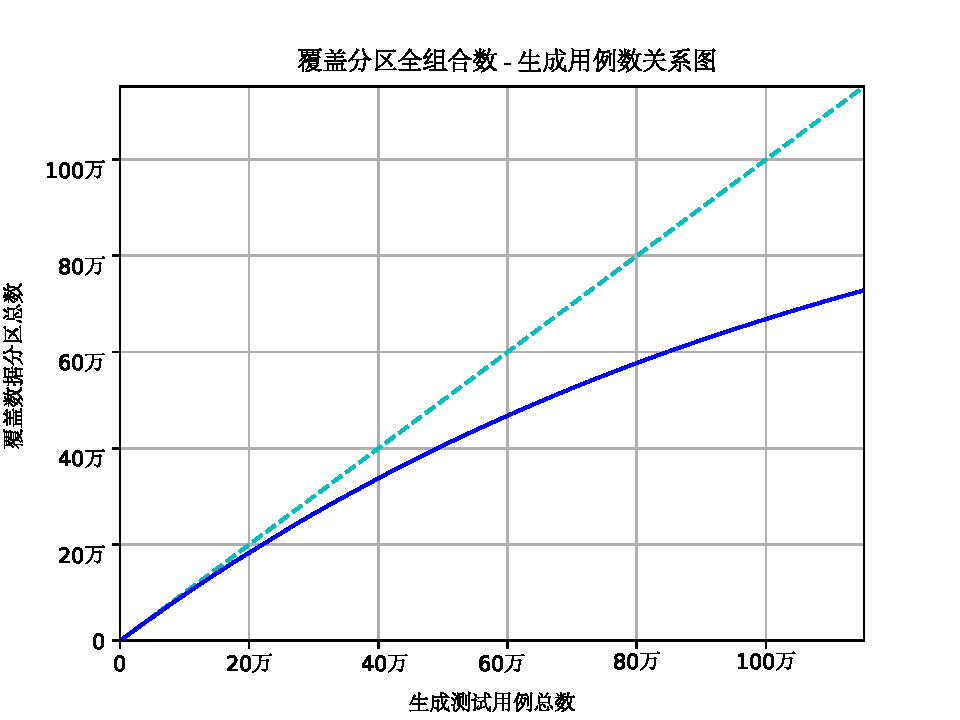
\includegraphics[width=200pt]{webank1_cn.pdf}
                    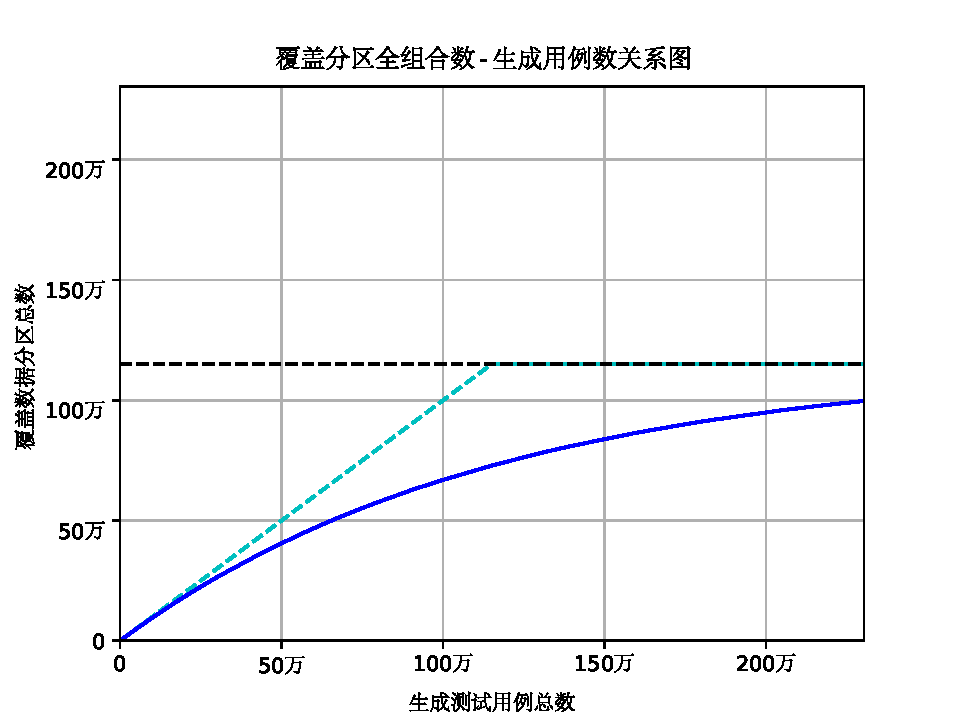
\includegraphics[width=200pt]{webank2_cn.pdf}
                    \caption[覆盖分区全组合数 - 生成用例数关系图]{覆盖分区全组合数 - 生成用例数关系图. 图中, 实线表示实验结果; 青色虚线为$y=x$, 表示最理想情况, 即每个测试用例覆盖一个新的数据分区全组合; 黑色虚线表示数据分区的全组合总数(1,152,000). 两幅子图系同一实验, 仅绘图尺度不同.}
                    \label{fig:partition}
                \end{figure}
                
                实验共生成了逾200万个测试用例, 图\ref{fig:partition}反映了生成的测试用例数目与它们覆盖的分区全组合数目之间的关系. 在图中, 青色虚线表示最理想的测试用例生成方法, 即每个新生成的测试用例均覆盖一个新的数据分区全组合; 黑色虚线表示数据分区的全组合总数(1,152,000); 蓝色实线表示在本文的场景模型上运行组合测试策略的实验结果. 两幅子图为同一实验, 但绘图尺度不同, 左图反映测试用例数目不超过数据分区全组合总数目时的趋势, 右图则反映测试用例数目不超过数据分区全组合总数目\textbf{两倍}时的趋势.
                
                当生成的测试用例数等于总数据分区全组合数(1,152,000)时, 覆盖的全组合数为728,239, 数据分区组合覆盖率为63.2\%. 当测试用例数为总数据分区全组合数的两倍时, 覆盖数增加至996,642, 对应覆盖率为86.5\%. 此结果说明, 使用本文的场景模型实现组合测试策略时, 如果生成测试用例数与总数据分区全组合数为同一数量级, 测试用例便可以覆盖大部分数据分区全组合, 因此是十分有效的.

                \vspace{1em}

                实际上, 在此场景模式上运行组合测试策略生成测试用例, 可以等价于在所有数据分区全组合构成的集合上进行放回的完全随机抽样. 使用$n$表示此集合的元素个数($n = |S|$), 使用$E(m)$表示经过$m$次抽样后, 抽到的不同元素数目的期望.
    
                则$E(m)$满足
                \begin{equation*}
                    \left\{
                    \begin{array}{l}
                         E(0) = 0; \\
                         E(m) = E(m-1) + \dfrac{n - E(m-1)}{n}, m > 0.
                    \end{array}
                    \right.
                \end{equation*}
                则有
                \begin{equation*}
                    \begin{aligned}
                        E(m) & =\left(\dfrac{n-1}{n}\right)^{0} + \cdots + \left(\dfrac{n-1}{n}\right)^{m-1} \\
                        & = n\left(1-(\dfrac{n-1}{n})^{m}\right).
                    \end{aligned}
                \end{equation*}
                
                令$k = \dfrac{m}{n}$, 则有$\dfrac{E(m)}{n} = 1 - \left(\dfrac{n-1}{n}\right)^{n\cdot k}$. 由于$\lim_{n\to\infty} \left(\dfrac{n-1}{n}\right)^n = \lim_{n\to\infty} \dfrac{1}{\left(1+\dfrac{1}{n-1}\right)^n} = \dfrac{1}{e}$, 可得$\lim_{n\to\infty}\dfrac{E(m)}{n} = 1 - \dfrac{1}{e^{k}} = 1 - \dfrac{1}{e^\frac{m}{n}}$.
                
                当$m=n$时, $E(m) = 1 - 1 / e = 63.2\%$. 当$m=2n$, $\lim_{n\to\infty} E(m) = 1 - 1 / e^2 = 86.5\%$. 均与实验结果相符.
    
        \subsection{故障检测能力}
        
            软件测试中, 一项基本的任务便是发现被测系统的故障与错误. 一个有实际应用价值的测试方法应能有效检测出系统故障.
            
            \begin{table}[!htb]
                \centering
                \begin{tabular}{lc}
                    \toprule
                    类型 & 占比 \\
                    \midrule
                    未写明的参数约束 & 15\% \\
                    未进行的输入检查 & 10\% \\
                    功能实现不完全 & 25\% \\
                    功能实现错误 & 5\% \\
                    被忽略的参数 & 5\% \\
                    不符合格式定义的响应 & 15\% \\
                    致命错误, 系统崩溃 & 25\% \\
                    \bottomrule
                \end{tabular}
                \caption[OSS系统中被检测出的故障的分类表]{OSS系统中被检测出的故障的分类. 此表说明, 各种类型的故障均可以被本文的测试方法自动有效检出.}
                \label{tab:oss_bug_classification}
            \end{table}
            
            在OSS系统的实验中, 根据自动化生成的测试用例的反馈结果, 本工作成功发现并确认了20个系统的真实故障. 故障的具体分类见表\ref{tab:oss_bug_classification}. 其中, 65\%的故障是在编写简单场景验证API基本行为时发现的, 35\%的故障是在三个综合场景中发现的.
            
            而在来自工业界的ECS服务上, 实验生成的100个测试用例则检测出了以下异常与故障:
            \begin{itemize}
                \item 对于删除实例(“DeleteInstance”)的API请求, 依照文档描述, 只要当前实例处于停止状态, 操作即可成功. 但是, 实际测试发现, 当实例已经处于停止状态几秒钟后, 此请求仍然失败并返回403状态码. 由于几秒钟的延迟较小, 人工测试难以发现, 可能是此故障遗留至今的原因.
                
                \item 实例的状态域有许多中间的过渡态没有在API文档中描述. API文档只记录了“Running”和“Stopped”态, 实际上还有“Creating”, “Starting”和“Stopping”这些过渡状态.
                
                \item 停止实例(“StopInstance”)的API行为不稳定. 当“ForceStop”参数设定为真时, 正常情况下, 几秒钟内实例即被停止, 并对用户发出响应, 但是, 偶尔, 此操作需要数分钟时间完成, 从而导致测试用例抛出响应超时异常.
                
                \item 绝大多数情况下, 创建实例(“CreateInstance”)的API响应时间在1秒以内, 但是, 偶尔, 响应时间需约10秒, 从而导致测试用例抛出响应超时异常.
            \end{itemize}
            
            另外, 为了对测试用例在故障检测方面的能力进行定量分析, 本文使用图\ref{fig:scenario_example}所示的场景模型, 在对应的小型实验系统上进行了故障检测能力实验.
            
            实验的设定为, 在实验系统的浏览微博API("ViewPost", 与$q_4$状态关联)中故意插入一个故障: 请求存在的微博时, 有$P_{bug}$的概率, 它故意返回"请求的微博不存在"的异常信息. 然后, 使用此场景模型随机生成并执行100个测试用例, 统计有多少比例的测试用例执行失败, 作为测试用例执行失败的概率的估计$P_{fail} = \# fail / 100$. 保证实验系统不存在其他故障, 因此测试用例执行失败均意味着这一故障被检测出, 因此$P_{fail}$亦为(仅生成一个测试用例时)故障的被发现概率. 如图\ref{fig:pbug_pfail_graph}即为故障的发现概率$P_{fail}$与故障的发生概率$P_{bug}$的关系曲线.
            \begin{figure}[!htb]
                \centering
                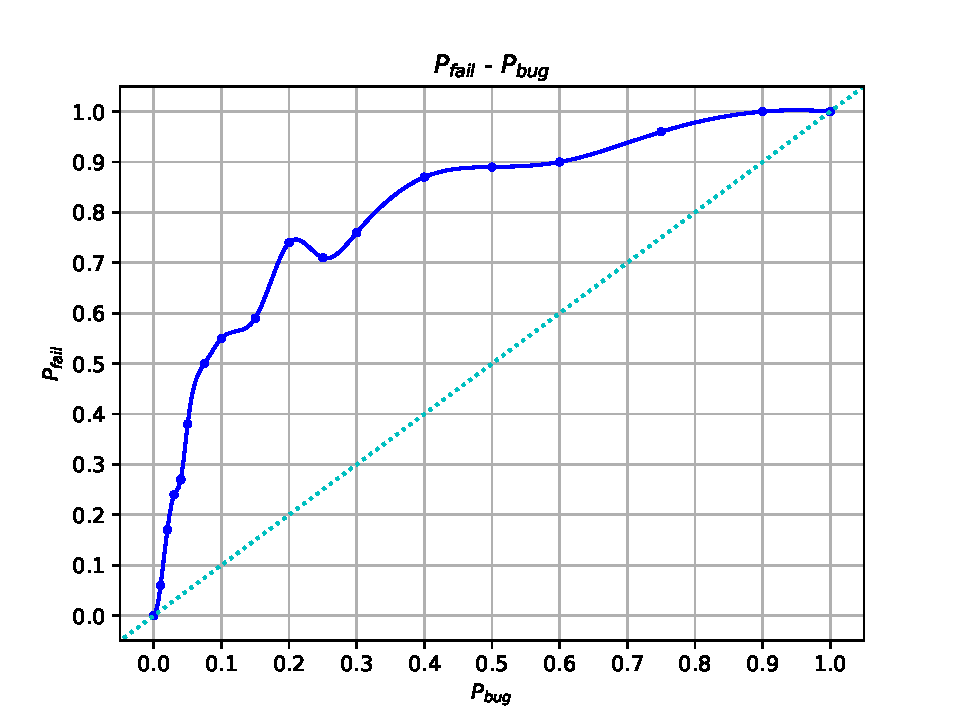
\includegraphics[width=400pt]{small_curve.pdf}
                \caption[故障的发现概率$P_{fail}$与发生概率$P_{bug}$的关系]{故障的发现概率$P_{fail}$与故障的发生概率$P_{bug}$的关系. 用蓝色实线表示. 青色虚线为单位线, 亦表示单API测试时此故障的发现概率.}
                \label{fig:pbug_pfail_graph}
            \end{figure}
            曲线表明, 使用此场景模型和测试生成方法, 即便仅生成一个测试用例, 故障的发现概率都要远远高于故障的发生概率. 说明使用此自动化测试方法具有较强的故障检测能力. 其原因为, 自动化生成的测试用例是复杂多样的API请求序列, 覆盖率和多样性方面较之简单测试方法有明显优势, 发现故障的可能性也就更大.
            
            以上实验结果表明, 本文的场景模型和自动化测试方法可以有效检出系统的故障和错误, 具有实际应用价值.
    
        \subsection{测试效率}
    
            进行自动化测试的一项重要初衷, 便是提高测试效率, 节省人工时间成本. 本工作用实验和量化分析粗略地分析了本文测试方法的测试效率.
            
            随着如OpenAPI的API行为规范描述语言的快速发展和流行, 在接口设计阶段提供公开的Web API描述脚本变得越来越常见. 因此, 在软件测试阶段, 使用本文的方法, 只需要设计场景模型即可.
            
            \begin{table}[!htb]
                \centering
                \small
                \begin{tabular}{ccc|ccc|c}
                    \toprule
                    \multirow{2}{*}{场景} & 场景脚 & 估计设 & 估计对应     & 估计   & 估计设     & 估计时间  \\
                                          & 本大小     & 计耗时                        & 测试脚本个数 & 脚本总大小 & 计耗时 & 节省率 \\
                    \midrule
                    Scenario A & 9.1 KB & 4.55 h & 4 & 12 KB & 6 h & 24.17\% \\
                    Scenario B & 9.6 KB & 4.80 h & 5 & 15 KB & 7.5 h & 36.00\% \\
                    Scenario C & 15.3 KB & 7.65 h & 8 & 24 KB & 12 h & 36.25\% \\
                    \bottomrule
                \end{tabular}
                \caption[OSS服务中场景设计估计耗时与人工脚本设计估计耗时对比表]{OSS服务三个综合测试场景的估计设计耗时以及与传统人工方法估计设计耗时的对比.}
                \label{tab:efficiency_esti}
            \end{table}
            
            在覆盖的功能点意义上, 每个场景模型可以等价于多个手工编写的测试脚本. 以OSS服务的三个综合场景Sceanrio A、 Scenario B和Scenario C为例, 根据功能点等价的原则, 本实验对每个测试场景等价的手工测试脚本数进行了较准确的估算. 公平起见, 估算时假设场景模型脚本和测试脚本均是纯人工编写的, 虽然使用\ref{sec:scenario_build}小节讨论的模型构建方法, 场景模型还可交互式构建和自动化构建. 如果人工编写测试脚本描述测试用例, 需要一定量的代码处理被测系统的启动/终止, 以及一定量的代码处理网络协议, 因此估计人工测试脚本的平均大小至少为3KB(约80行). 然后, 假设对于有经验的测试人员, 每2KB(约50行)脚本/代码的编写和调试时间为1小时. 有了这些数据, 即可估算自动化测试方法与人工测试方法所需的人工设计总耗时, 估算结果见表\ref{tab:efficiency_esti}.
            
            从表\ref{tab:efficiency_esti}中可以看出, 相比人工测试, 本文提出的自动化测试方法的效率提高直接反映在需要手工编写的脚本大小的减少, 这个减少在24\%到37\%之间. 此外, 场景模型交互式构建和自动化构建方法的引入将进一步显著提高基于场景模型的自动化测试的效率. 总而言之, 根据以上科学估计, 可以得知, 使用本文的自动化测试方法可以有效节省人工时间成本, 提高测试效率.

        \subsection{小结}
            通过以上实验与评估, 我们验证了本文的场景模型和自动化测试方法可以生成多样化的测试用例, 达到较高的覆盖率, 并且有能力检测出实际系统中存在的故障, 同时显著提高测试的效率, 减少成本. 具有研究与应用价值.
